The software outputs seven files: five sensor data files, a metadata file, and a file containing time stamps and labels.
The file names and a general description of the content is documented in Table \ref{tab:3-files}.

\begin{table}[H]
    \centering
    \begin{tabular}{l l}
    \toprule
    \textbf{File name} & \textbf{Description} \\
    \midrule
    audio.wav & Microphone samples \\
    depth.raw & Depth camera record \\
    ir.raw & \gls{ir} camera record \\
    metadata.yaml & Metadata \\
    radar.raw & Radar samples \\
    rgb.raw & RGB camera record \\
    timestamps.csv & Activity labels and time stamps \\
    \bottomrule
    \end{tabular}
    \caption{Files output by the software}
    \label{tab:3-files}
\end{table}

The sensor data files contain unprocessed (raw) data outputted by the sensors;
only the data in \texttt{ir.raw} has been repacked into a different number format.
To extract meaningful data from the files, the file formats must be understood.
Additionally, it may be beneficial to perform some post-processing for the data,
especially in the case of the \texttt{radar.raw} file.

The following sections will document the exact formats of the file
and present some relevant data processing algorithms for each data file format.

\section{Activity labels and time stamps}
The activity labels and their corresponding time stamps are stored in the file \texttt{timestamps.csv}.
As implied by the file name, the file follows the \gls{csv} format, delimited by the comma character (",", unicode U+002C).
The file contains two columns.
The first column contains time stamps and the second column contains labels.
Listing \ref{lst:labels} provides an example of the file.

\begin{lstlisting}[caption={Example \texttt{timestamps.csv} file.}\label{lst:labels}]
    0.000506,sitting
    1.689381,stand_up
    4.106970,walking
    7.184435,pick
    9.060120,walking
    12.494,STOP
\end{lstlisting}

The activities are sorted by time in an ascending order.
The time stamps tell the time elapsed since the beginning of the recording.
The frame rate for each sensor is recorded in the \texttt{metadata.yaml} file.
Based on the timestamps and the frame rate of each sensor, the mapping between frames and labels can be made.
The time of recording $t_{\mathrm{min}}$, $t_{\mathrm{max}}$ for a given frame can be calculated via equation \ref{eq:frame-number-to-time},
where $N_{s}$ is the sampling rate of the sensor and $n$ is the frame number.

\begin{equation}
    \label{eq:frame-number-to-time}
    \begin{cases}
        t_{\mathrm{min}} = \frac{n}{N_{s}} \\
        t_{\mathrm{max}} = \frac{n+1}{N_{s}}
    \end{cases}
\end{equation}

Given $t_{\mathrm{min}} \leq T < t_{\mathrm{max}}$, where $T$ is the timestamp of an activity, the activity should be mapped to the frame.

\section{IR camera record}
\label{sec:ir-file}
The frames produced by the infrared block consist of 64 numbers (8x8 pixels).
The frames are stored in the \texttt{ir.raw} file.
Each pixel is represented by a half-precision (16-bit) floating point number.
The values represent the recorded temperatures in each pixel.

The pixels of each frame are stored in row-major order,
thus denoting the vector containing the recorded values as $\vec{d}$,
the frames can be represented by equation $\ref{eq:ir-frame}$,
where $\vec{F}_{z}$ is the $z$:th frame, $n$ is the row of a pixel and $m$ is the column of a pixel.

\begin{equation}
    \label{eq:ir-frame}
    \forall n \in [0, 7] \land m \in [0, 7] \land j \in \left[ 0, \frac{|d|}{64} \right] : \vec{F}_{z}(n, m) = \vec{d}(64z+8n+m)
\end{equation}

The origin of the image is in the upper left corner.
Figure \ref{fig:ir-orig} shows an example frame parsed from the file and \ref{fig:ir-rgb} shows the corresponding RGB image.
The data in frame $\vec{F}_z$  may be used as-is, but the resolution of the image may be increased by interpolating.
Figures \ref{fig:ir-interp-2x} and \ref{fig:ir-interp-4x} illustrate the effects of increasing the resolution of the original image
to 16x16 and 32x32 using cubic interpolation.
A code example in Python for parsing the frames from the file is given in Appendix \ref{app:ir-parsing}.

\begin{figure}[H]
    \centering
    \begin{subfigure}[b]{0.475\textwidth}
        \centering
        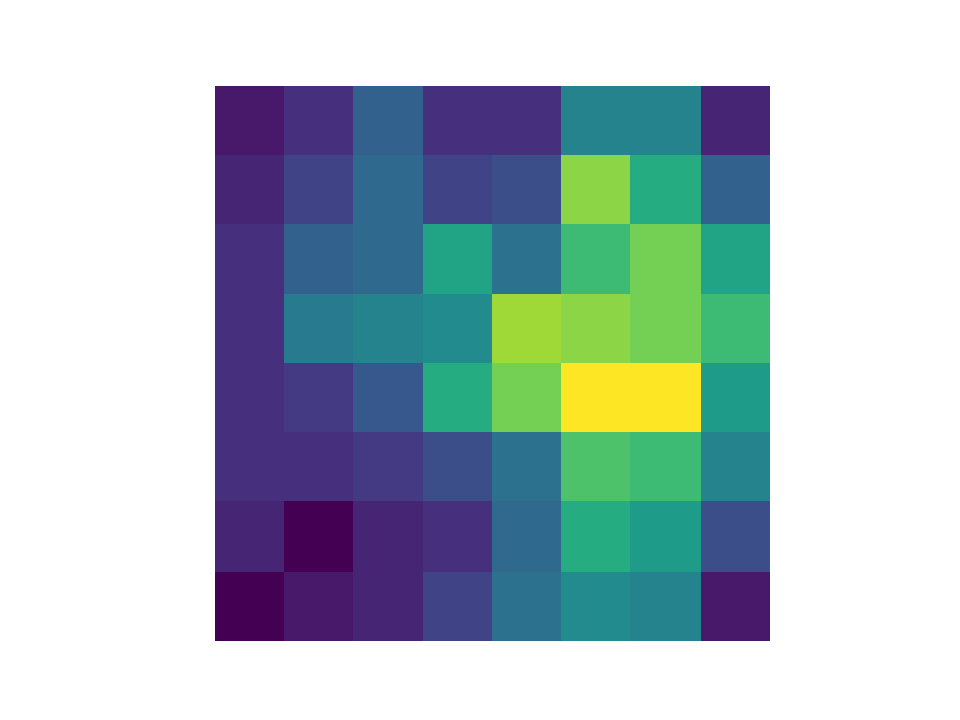
\includegraphics[width=\textwidth]{fig/4/ir-orig.pdf}
        \caption{Original 8x8 image}
        \label{fig:ir-orig}
    \end{subfigure}
    \hfill
    \begin{subfigure}[b]{0.475\textwidth}
        \centering
        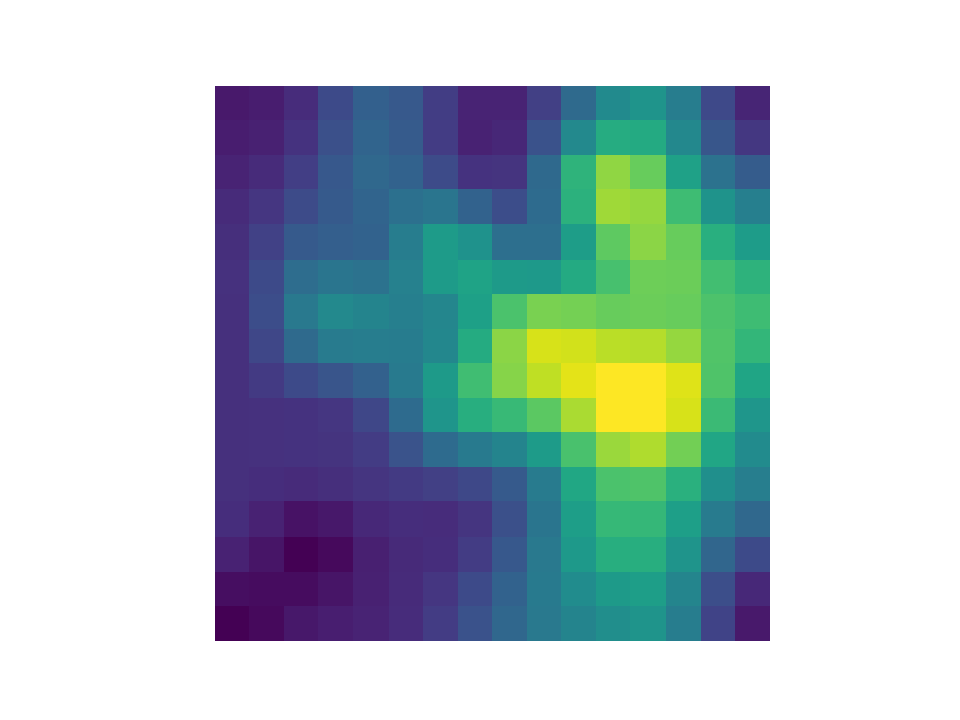
\includegraphics[width=\textwidth]{fig/4/ir16.pdf}
        \caption{Upscaled 16x16 image}
        \label{fig:ir-interp-2x}
    \end{subfigure}
    \vskip\baselineskip
    \begin{subfigure}[b]{0.475\textwidth}
        \centering
        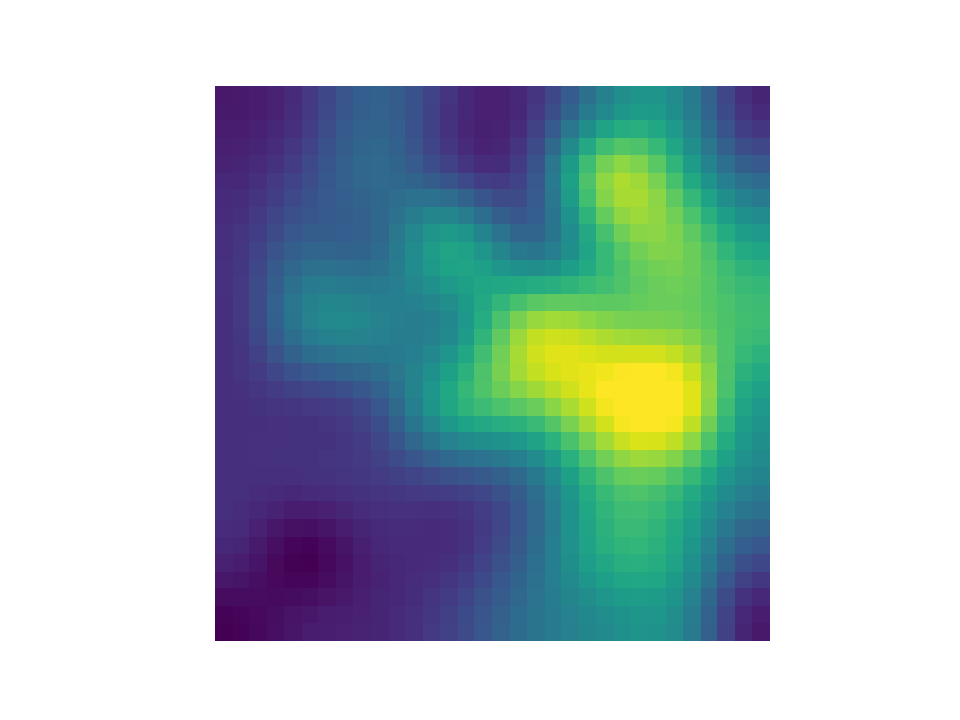
\includegraphics[width=\textwidth]{fig/4/ir32.pdf}
        \caption{Upscaled 32x32 image}
        \label{fig:ir-interp-4x}
    \end{subfigure}
    \hfill
    \begin{subfigure}[b]{0.475\textwidth}
        \centering
        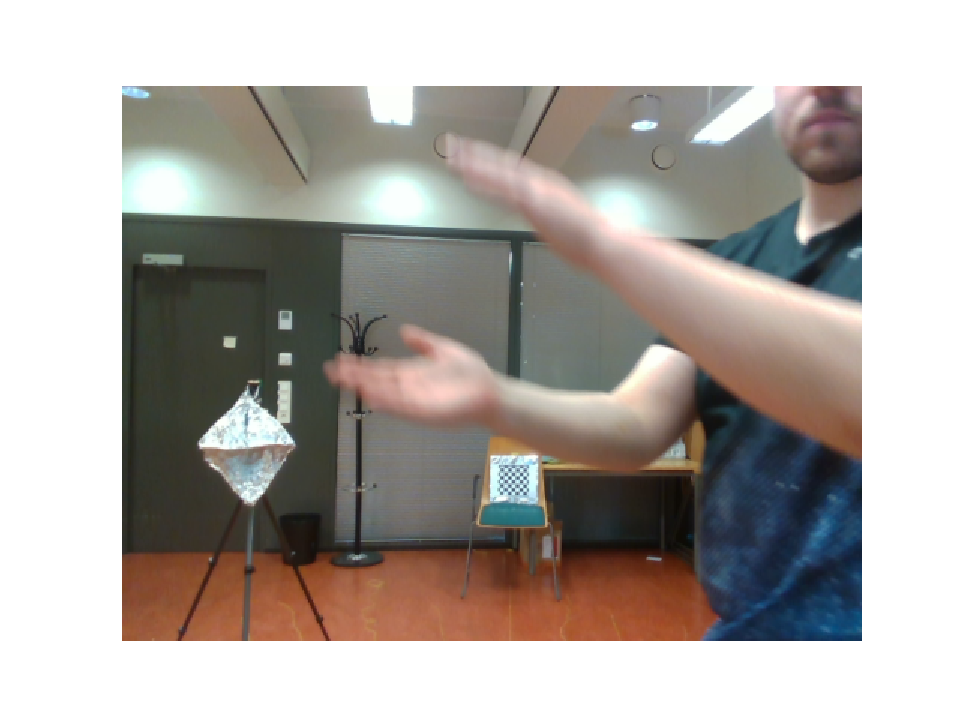
\includegraphics[width=\textwidth]{fig/4/ir-rgb.pdf}
        \caption{Corresponding RGB image}
        \label{fig:ir-rgb}
    \end{subfigure}
    \caption{An \gls{ir} frame interpolated to different higher resolutions and the corresponding RGB frame.}
    \label{fig:ir-interpolated}
\end{figure}

\section{Radar samples}
\label{sec:radar-file}
The Texas Instruments mmWave Radar Device ADC Raw Data Capture application report defines multiple data formats for the DCA1000EVM data output format,
which is also the format the data is stored in the \texttt{radar.raw} file \cite{dca1000-raw-data-capture}.
Combined with the TI6843ISK radar module, the data formats are limited to only one option \cite{mmwave-sdk-user-guide}.
The data is sampled in the \gls{iq} format.
Given there are $N$ samples per chirp, $M$ chirps per frame, and $K$ active receivers,
the data can be arranged to radar cubes and frames via the procedure explained in Section \ref{sec:radar-data}.

After the raw data has been rearranged into radar cubes and frames of complex data,
numerous radar processing algorithms can be applied to the data to extract valuable information about the targets.
Algorithms for detecting targets in the range-azimuth domain and obtaining time-doppler spectra for the targets are presented in Section \ref{sec:radar-processing}.

Throughout this section, the symbols listed in Table \ref{tab:radar-symbols} are used.
The values represented by the symbols are stored in the \texttt{metadata.yaml} file
under the \texttt{radar} section.
The keys that correspond to the values of the symbols and the meanings of the symbols, are also listed in the table.

\begin{table}[h]
    \centering
    \begin{tabular}{c l p{3in}}
    \toprule
        \textbf{Symbol} & \textbf{Key} & \textbf{Meaning} \\
    \midrule
         $N$ & samples\_per\_chirp & Number of samples per chirp \\
         $M$ & chirps\_per\_frame & Number of chirps per frame \\
         $K$ & num\_channels & Number of active receivers \\
         $T_c$ & chirp\_cycle\_time & Time between each frame [s] \\
         -- & framerate & Number of frames (radar cubes) recorded per second [Hz] \\
         $F_s$ & samplerate & Sampling frequency in the receivers [Hz] \\
         $S$ & slope & Slope of the transmitted chirp [Hz/s] \\
    \bottomrule
    \end{tabular}
    \caption{
        Symbols used throughout this section, their corresponding keys in the \texttt{metadata.yaml} file and their meanings.
        Framerate is not used in this section, thus it has no symbol.
    }
    \label{tab:radar-symbols}
\end{table}

\subsection{Radar file format}
\label{sec:radar-data}

Based on the metadata, the raw samples in the \texttt{radar.raw} file can be rearranged into radar cubes.
Each radar cube consists of $N \times M \times K$ complex samples as illustrated in Figure \ref{fig:radar-cube}
Each complex sample in the raw data consists of two values: the in-phase and the quadrature component.
Both components are represented as 16-byte integers in the raw data.

Denoting the raw 16-byte integer samples as $\vec{d}$, the real (in-phase) and imaginary (quadrature) components
of the complex samples can be extracted with the following formulas:

\begin{equation}
    \forall x \in \left[ 0, \frac{|d|}{2} \right] \begin{split}
        \begin{cases}
            \vec{d}_r(x) = \vec{d}(4x) \\
            \vec{d}_i(x) = \vec{d}(4x+2)
        \end{cases} ,\bmod(n, 2) = 0 \\
        \begin{cases}
            \vec{d}_e(x) = \vec{d}(4x+1) \\
            \vec{d}_i(x) = \vec{d}(4x+3)
        \end{cases} ,\bmod(x, 2) \neq 0
    \end{split}
\end{equation}

where $\vec{d}_{r}(x)$ is the $x$:th element of the vector containing the real samples,
and alike, $\vec{d}_{i}(x)$ is the $x$:th element of the vector containing the imaginary samples.
Thus, the vector containing the complex samples $\vec{s}$ is given by equation \ref{eq:complex-samples}, where $j$ is the imaginary unit.

\begin{equation}
    \label{eq:complex-samples}
    \vec{s} = \vec{d}_{r} + j\vec{d}_{i}
\end{equation}

Each $N \times M \times K$ elements of $\vec{s}$ constitute a single radar cube.
The samples for the $z$:th cube (or frame), denoted as $\vec{s}_{z}$, can be extracted from $\vec{s}$ as given by equation \ref{eq:z-samples} 

\begin{equation}
    \label{eq:z-samples}
    \vec{s}_{z} = \begin{bmatrix} \vec{s}(zNMK) & \vec{s}(zNMK+1) & \ldots & \vec{s}(zNMK+(NMK-1)) \end{bmatrix} ^{T}
\end{equation}

Each radar cube consists of $M \times K$ chirps, whereas each chirp consists of $N$ samples.
Each $N$ samples in $\vec{s}$ constitutes for a chirp, thus the $m$:th chirp in $\vec{s}_{z}$, i.e. $\vec{c}_{m}$, is given by equation \ref{eq:c_m}.

\begin{equation}
    \label{eq:c_m}
    \vec{c}_{m} = \begin{bmatrix} \vec{s}_{z}(mN) & \vec{s}_{z}(mN+1) & \ldots & \vec{s}_{z}(mN+(N-1))  \end{bmatrix} ^T
\end{equation}

The chirps are organized in such way in the data that each $K$ chirps are sampled at the same time,
but in different receivers.
Thus, the frame $\vec{s}_{z}$ can be reshaped into a tensor $\vec{S}_{z}$ via the transformation given by equation \ref{eq:transformation}.

\begin{equation}
    \label{eq:transformation}
    \vec{S}_{z} =
        \begin{bmatrix}
            \vec{c}_{0}   & \vec{c}_{K}    & \vec{c}_{2K} & \ldots & \vec{c}_{(M-1)K}   \\
            \vec{c}_{1}   & \vec{c}_{K+1}  & \vec{c}_{2K+1} & \ldots & \vec{c}_{(M-1)K+1} \\
            \vdots        & \vdots         & \vdots       & \ddots & \vdots             \\
            \vec{c}_{K-1} & \vec{c}_{2K-1} & \vec{c}_{3K-1} & \ldots & \vec{c}_{MK-1}
        \end{bmatrix}
\end{equation}

For each sample in $\vec{S}_z$ that has the same first dimension index has an equal sampling time.
The sampling time increases by $T_c$ for each index in the second dimension of $\vec{S}_z$ and 
by $\Delta t$ for each index in the third dimension.
The third dimension is the index of the vectors $\vec{c}_m$.
The dimensions of the tensor $\vec{S}_z$ are therefore equal to the radar data cube presented in Figure \ref{fig:radar-cube}.

\begin{figure}
    \centering
    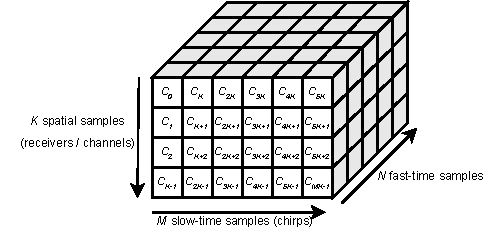
\includegraphics[width=0.9\textwidth]{fig/4/radar-cube.pdf}
    \caption{Radar cube with dimensions corresponding to $\vec{S}_y$.}
    \label{fig:radar-cube}
\end{figure}

Using the described transformations, the vector $\vec{s}$ can be transformed into a 4-dimensional tensor $\vec{S}$

\begin{equation}
    \vec{S} = \begin{bmatrix} \vec{S}_0 & \vec{S}_1 & \vec{S}_2 & \ldots & \vec{S}_Y & \end{bmatrix}^T,
\end{equation}

where $Y = | \vec{s} | \div (NMK)$ is the number of recorded frames.
The Appendix \ref{app:get_frames} presents an example of parsing the tensor $\vec{S}$ from the \texttt{radar.raw} file using Python and Numpy.

To turn the radar data cubes into useful information,
multiple data processing algorithms can be applied to the data.
Since most \gls{har} methods for radar signals use the Doppler-spectrum,
the most interesting information is the target positions and the Doppler spectra \cite{sensing-survey}.
The position information can be used to track the targets and get continuous time-Doppler data for a given target.
Additionally, the position information can be used to aid in the microphone beam forming.

Section \ref{sec:range-angle} briefly covers the methods for extracting the range-azimuth information from the radar samples.
Section \ref{sec:cfar} briefly covers the methods for detecting and tracking targets from the data,
and finally, Section \ref{sec:doppler-spectrum} briefly covers the \gls{fft} based algorithm for extracting the Doppler-spectrum.

\subsection{Range-azimuth spectrum}
\label{sec:range-angle}

For extracting the range-azimuth data from the radar signals,
\gls{2d-music} is one of the most attractive methods.
Compared to the traditional \gls{fft} based methods, the \gls{2d-music} can achieve significantly better resolution
in both the angular domain and the range domain \cite{2d-music-van-rossum}.
A major downside of the \gls{2d-music} algorithm is extremely high computational load and memory usage.
The use of \glspl{fpga} or \glspl{asic} may be used in applications to make the computations faster.

The radar device used in the sensor assembly can be configured to switch between two transmitting antennas,
such that odd chirps are transmitted on a different antenna than even chirps.
If this feature is used, the effective amount of spatial channels in the radar data is $2K$,
and each two radar cubes can be combined along the first axis to form another data cube.\cite{ti-iwr-user-guide}
Based on this, a new tensor $\vec{S}^\prime$ can be defined along a new variable $K^\prime$ that is the number of active receivers.

\begin{align}
    &\begin{cases}
        \vec{S}^{\prime}(z) = (\vec{S}(2z) | \vec{S}(2z+1)) \\
        K^\prime = 2K
    \end{cases}&,~\mathrm{if~switching~between~transmitters}
    \\
    &\begin{cases}
        \vec{S}^{\prime}(z) = \vec{S}(z) \\
        K^\prime = K
    \end{cases}&,~\mathrm{othwerwise}
\end{align}

The tensor augmentation operation $(\vec{A} | \vec{B})$ is defined by the transformation \\
$(\vec{A}^{K \times N \times M}, \vec{B}^{K \times N \times M}) \to \vec{(A|B)}^{2K \times N \times M}$, given by
equation \ref{eq:tensor-augmentation} where the magnitude of each element $|~(\vec{A}|\vec{B})(k, n)~| = M$.

\begin{equation}
\label{eq:tensor-augmentation}
    (\vec{A} | \vec{B}) =
    \begin{bmatrix}
        \vec{A}(0, 0) & \vec{A}(0, 1) & \ldots & \vec{A}(0, M) \\
        \vec{A}(1, 0) & \vec{A}(1, 1) & \ldots & \vec{A}(1, M) \\
        \vdots        & \vdots        & \ddots & \vdots        \\
        \vec{A}(K, 0) & \vec{A}(K, 1) & \ldots & \vec{A}(K, M) \\
        \vec{B}(0, 0) & \vec{B}(0, 1) & \ldots & \vec{B}(0, M) \\
        \vec{B}(1, 0) & \vec{B}(1, 1) & \ldots & \vec{B}(1, M) \\
        \vdots        & \vdots        & \ddots & \vdots        \\
        \vec{B}(K, 0) & \vec{B}(K, 1) & \ldots & \vec{B}(K, M) \\
    \end{bmatrix},
\end{equation}

Using these definitions, the \gls{2d-music} spectrum can be calculated.
The first and third dimension of the tensor $\vec{S}^{\prime}$ constitute for the samples recorded during a single dwell,
i.e. a chirp. It can be represented by the tensor $\vec{D}_m$, given by equation \ref{eq:tensor-D}.
The part of the data cube represented by $\vec{D}_m$ is highlighted in Figure \ref{fig:tensor-D}.

\begin{equation}
\label{eq:tensor-D}
    \vec{D}_m = \begin{bmatrix} \vec{S}^{\prime}(0, m) & \vec{S}^{\prime}(1, m) & \ldots & \vec{S}^{\prime}(K^{\prime}, m)  \end{bmatrix} ^T
\end{equation}

\begin{figure}[H]
    \centering
    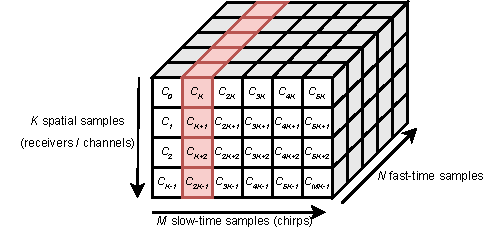
\includegraphics[width=0.9\textwidth]{fig/4/radar-cube-tensor-D.pdf}
    \caption{The part of the radar data cube represented by the tensor $\vec{D}_m$ is highlighted in red ($m = 1$).}
    \label{fig:tensor-D}
\end{figure}

Under the narrowband assumption, the samples of the tensor $\vec{D}_m$ can be modeled
as given by equation \ref{eq:sample-approximation} \cite{music-based-algo}.
The symbols used in the equation  are defined in Table \ref{tab:sample-approximation-variables}.

\begin{equation}
\label{eq:sample-approximation}
\vec{D}_{m} (k, n) =
    \sum_{l=0}^{L-1} \alpha_{l} e^{j \phi_{l}} ~
        e^{j 2 \pi \frac{2 R_{l} \Delta F}{c T} n \Delta t } ~
        e^{ j \frac{2 \pi}{ \lambda } d k \sin \theta_{l}}
        + \omega(k, n).
\end{equation}

\begin{table}[]
    \centering
    \begin{tabular}{c l l}
    \toprule
        \textbf{Symbol} & \textbf{Definition} \\
    \midrule
        $k$ & Index of an antenna in the receiving uniform linear array \\
        $n$ & Index of a fast-time sample in $\vec{c}_z$\\
        $L$ & Number of reflecting radar targets \\
        $\alpha_{l}$ & Amplitude of the reflected signal from the $l$:th target \\
        $e^{j \phi_{l}}$ & Phase of the reflected signal from the $l$:th target\\
        $R$ & Range from the receiver to the $l$:th target \\
        $\Delta F$ & The bandwidth of the signal during the sampling time \\
        $\Delta t$ & Sampling time: inverse of the sampling frequency \\
        $c$ & The speed of light \\
        $T$ & Dwell time: $N \Delta t$\\
        $\theta_{l}$ & Angle of arrival of the signal reflected from the $l$:th target \\
        $\omega(k, n)$ & Additive white Gaussean noise in the $n$:th sample of the $k$:th receiver \\
    \bottomrule
    \end{tabular}
    \caption{Definitions of the symbols used in equation \ref{eq:sample-approximation}.}
    \label{tab:sample-approximation-variables}
\end{table}

The tensor $\vec{D}_m$ also be represented in matrix format as shown by the equations 
\ref{eq:matrix-sample-approximation-1}--\ref{eq:matrix-sample-approximation-6}.

\begin{align}
\label{eq:matrix-sample-approximation-1}
    &\vec{D}_m = \vec{A}\vec{X}\vec{R} + \vec{W} \\
\label{eq:matrix-sample-approximation-2}
    &\vec{A} = \begin{bmatrix} \vec{a}(\theta_0) & \vec{a}(\theta_1) \ldots & \vec{a}(\theta_{L-1}) \end{bmatrix}_{K \times L} \\
\label{eq:matrix-sample-approximation-3}
    &\vec{X} = \begin{bmatrix} \alpha_{0}~e^{j\phi_{0}} & & & \\ & \alpha_{1}~e^{j\phi_{1}} & & \\ & & \ddots & \\ & & & \alpha_{L-1}~e^{j\phi_{L-1}} \end{bmatrix}_{L \times L} \\
\label{eq:matrix-sample-approximation-4}
    &\vec{R} = \begin{bmatrix} \vec{r}(R_0) & \vec{r}(R_1) \ldots & \vec{r}(R_{L-1}) \end{bmatrix}_{N \times L} \\
\label{eq:matrix-sample-approximation-5}
    &\vec{a}(\theta_l) = \begin{bmatrix} 1 & e^{ j \frac{2 \pi}{ \lambda } d \sin \theta_{l}} & \ldots  & e^{ j \frac{2 \pi}{ \lambda } d(K-1) \sin \theta_{l}} \end{bmatrix}_{1 \times K}^{T} \\
\label{eq:matrix-sample-approximation-6}
    &\vec{r}(R_l) = \begin{bmatrix} 1 & e^{j 2 \pi \frac{2 R_{l} \Delta F}{c T} \Delta t } & \ldots & e^{j 2 \pi \frac{2 R_{l} \Delta F}{c T} (N-1) \Delta t } \end{bmatrix}_{1 \times N}
\end{align}

Equation \ref{eq:matrix-sample-approximation-1} is equivalent to equation \ref{eq:sample-approximation}.
In equation \ref{eq:matrix-sample-approximation-1}, $\vec{A}$ is the angle steering matrix consisting of the steering vectors $\vec{a(\theta_0)}$ ... $\vec{a(\theta_{L-1})}$.
The matrix $\vec{S}$ is the range steering matrix which consists of the range steering vectors $\vec{r}(R_0)$ ... $\vec{r}(R_{L-1})$.
The diagonal matrix $\vec{X}$ contains the complex amplitudes and phases of the reflected signals.
Finally, the $\vec{W}$ is the additive white Gaussean noise matrix.
Using this information, the \gls{2d-music} algorithm can be applied to calculate the range-azimuth spectrum.

The \gls{2d-music} algorithm is based on evaluation of the covariance matrix of the received signal and the separation of noise and target signal subspaces.
Multiple sweeps (chirps) are typically used for evaluating the covariance matrix.
The noise and target signal subspaces are estimated from the covariance matrix by applying eigenvalue decomposition to the covariance matrix.
The resulting eigenvalues are then used to estimate the number of targets to separate the subspaces.
The \gls{2d-music} spectrum is then estimated from the correlation of the noise subspace
and the range-azimuth steering matrix given by equation \ref{eq:steering-matrix}. \cite{2d-music-van-rossum}

When the reflected signals are correlated, which is the case when a target spans multiple range or angle bins,
the dimension of the signal subspace is not equal to the number of targets.
This can be solved by applying smoothing techniques, such as \gls{fbss}, to the data. \cite{2d-music-van-rossum, fbss-techniques}

For a $K^{\prime} \times N$ matrix, the \gls{fbss} algorithm is applied by defining a window with dimensions $q_1 \times q_2$,
and then scanning the data matrix in all possible positions: 
$p_1 = K^{\prime} - q_1$ positions in the angular dimension and $p_2 = N - m_2$ positions in the range dimension.
For each scanning position, the sub-matrix is flattened in column-major order to form the vector $\vec{d}(\tilde{p}_1, \tilde{p}_2)$,
where $\tilde{p}_2 \in \left[ 0, p_1 \right)$ and $\tilde{p}_2 \in \left[ 0, p_2 \right) $.
The vectors $\vec{d}(\tilde{p}_1, \tilde{p}_2)$ are then stacked column-wise to form the spatial-smoothed data matrix $\vec{\tilde{D}}_m$.
The scanning procedure is illustrated in Figure \ref{fig:data-matrix-scanning}. \cite{2d-music-van-rossum, music-based-algo}

\begin{figure}[H]
    \centering
    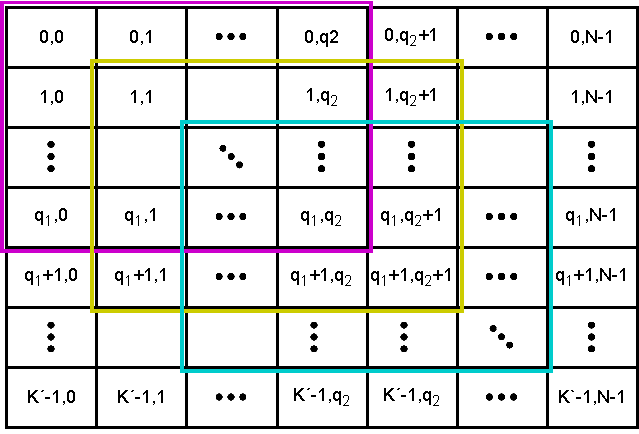
\includegraphics[width=0.67\textwidth]{fig/4/array-scanning.pdf}
    \caption{Scanning window procedure for the data matrix. The matrix is scanned in all possible positions where the $q_1 \times q_2$ window can fit.}
    \label{fig:data-matrix-scanning}
\end{figure}

\begin{equation}
\label{eq:fbss-scanning}
    \vec{\tilde{D}}_m = \begin{bmatrix}  \vec{d}(0, 0) & \vec{d}(1, 0) & \ldots & \vec{d}(p_{1}-1, 0) & \vec{d}(0, 1) & \vec{d}(1, 1) \ldots & \vec{d}(p_{1}-1, p_{2}-1) \end{bmatrix}
\end{equation}

The resulting dimensions of $\vec{\tilde{D}}_m$ are $q_{1}q_{2} \times p_{1}p_{2}$.
The vectors $\vec{d}(\tilde{p}_1, \tilde{p}_2)$ are given by equation \ref{eq:scanning}.

\begin{equation}
    \label{eq:scanning}
    \vec{d}(\tilde{p}_1, \tilde{p}_2) = \begin{bmatrix} 
        \vec{D}_{m}(\tilde{p}_{1}, \tilde{p}_{2}) \\
        \vec{D}_{m}(\tilde{p}_{1}+1, \tilde{p}_{2}) \\
        \vdots \\
        \vec{D}_{m}(\tilde{p}_{1}+q_{1}-1, \tilde{p}_{2}) \\
        \vec{D}_{m}(\tilde{p}_{1}, \tilde{p}_{2}+1) \\
        \vec{D}_{m}(\tilde{p}_{1}+1, \tilde{p}_{2}+1) \\
        \vdots \\
        \vec{D}_{m}(\tilde{p}_{1}+q_{1}-1, \tilde{p}_{2}+q_{2}-1)
    \end{bmatrix}_{q_{1}q_{2} \times 1}
\end{equation}

Having formed the smoothed data matrix $\vec{\tilde{D}}_m$, the data smoothed covariance matrix $C_{\tilde{D}_m}$ 
can then be evaluated as given by equation \ref{eq:covariance-matrix}.
The matrix $\vec{J}$ in equation \ref{eq:covariance-matrix} is the transition matrix defined by equation \ref{eq:transition-matrix}.
\cite{2d-music-van-rossum, fbss-techniques}

\begin{equation}
    \label{eq:covariance-matrix}
    \vec{C}_{\tilde{\vec{D}}_m} =
        \frac{1}{2 p_{1} p_{2} }
        \left[
            \vec{\tilde{D}}_{m} \vec{\tilde{D}}_{m}^{H}
            + \vec{J}(\vec{\tilde{D}}_{m} \vec{\tilde{D}}_{m}^{H})^{*}\vec{J} 
        \right]
\end{equation}

\begin{equation}
    \label{eq:transition-matrix}
    J = \begin{bmatrix}
        0      & 0      & \ldots & 1      \\
        \vdots & 0      & 1      & 0      \\
        0      & \iddots & 0      & \vdots \\
        1      & 0      & \ldots & 0      \\
    \end{bmatrix}_{q_{1}q_{2} \times q_{1}q_{2}}
\end{equation}

To estimate the signal and noise subspaces, the mean of the covariance matrices of multiple sweeps is used.
The final covariance matrix used for the eigenvalue decomposition is given by equation \ref{eq:mean-covariance-matrix}.
\cite{music-based-algo}

\begin{equation}
    \label{eq:mean-covariance-matrix}
    \vec{C}_{\tilde{\vec{D}}} = \frac{1}{M} \sum_{m=0}^{M-1} \vec{C}_{\tilde{\vec{D}}_m}
\end{equation}

The covariance matrix $\vec{C}_{\tilde{\vec{D}}}$ can be factorized as

\begin{equation}
    \vec{C}_{\tilde{\vec{D}}} = \vec{Q} \vec{\Lambda} \vec{Q}^{H},
\end{equation}

where $\vec{Q}$ contains the eigenvectors of $\vec{C}_{\tilde{\vec{D}}}$ and $\vec{\Lambda}$ is a diagonal matrix containing the corresponding eigenvalues.
Given the number of targets $L$ (equations \ref{eq:num-targets}--\ref{eq:music-mdl}),
the noise subspace $\vec{Q}_{n}$ with dimensions  $q_{1}q_{2} \times p_{1}p_{2} - L$
can be partitioned from $\vec{Q}$ as shown by equation \ref{eq:noise-subspace-partition} \cite{2d-music-van-rossum}.

\begin{equation}
    \label{eq:noise-subspace-partition}
    \vec{Q}_{n} = \begin{bmatrix} \vec{Q}(L) & \ldots & \vec{Q}(p_{1}p_{2} - 1) \end{bmatrix}
\end{equation}

The number of targets $L$ can be estimated using information theoretic criteria, such as \gls{aic} or \gls{mdl}.
As proposed by Wax and Kailath, equation \ref{eq:music-aic} shows the formula for \gls{aic} for this problem
and equation \ref{eq:music-mdl} shows the formula for \gls{mdl}.
For both equations, the number of targets is the argument of the minimum for the criteria (Equation \ref{eq:num-targets}).
\cite{wax-kailath-85}

\begin{equation}
    \label{eq:num-targets}
    L = \argmin\limits_{0\,\leq\,l\,<\,q_{1}q_{2}}\, \mathrm{AIC}(l) \quad \vee \quad L = \argmin\limits_{0\,\leq\,l\,<\,q_{1}q_{2}}\, \mathrm{MDL}(l)
\end{equation}

\begin{equation}
    \label{eq:music-aic}
    \mathrm{AIC}(l) = -2 \log \left(
        \frac
            {\prod\limits_{i = l}^{q_{1}q_{2}-1} \Lambda(i,i)^{1 \div (q_{1}q_{2} - l)}} 
            {\frac{1}{q_{1}q_{2}-k} \sum\limits_{i=l}^{q_{1}q_{2}-1} \Lambda(i,i)}
    \right)^{(q_{1}q_{2}-l)K} + 2l(2q_{1}q_{2}-k)
\end{equation}

\begin{equation}
    \label{eq:music-mdl}
    \mathrm{MDL}(l) = - \log \left( 
        \frac
            {\prod\limits_{i = l}^{q_{1}q_{2}-1} \Lambda(i,i)^{1 \div (q_{1}q_{2} - l)}} 
            {\frac{1}{q_{1}q_{2}-k} \sum\limits_{i=l}^{q_{1}q_{2}-1} \Lambda(i,i)}
    \right)^{(q_{1}q_{2}-l)K} + \frac{1}{2}l(2q_{1}q_{2}-l) \log K
\end{equation}

Having estimated the noise subspace, the \gls{2d-music} spectrum $\vec{P}(R, \theta)$ is given by equation \ref{eq:2d-music-spectrum}.
The range-azimuth steering matrix $\vec{V}(\theta, R)$ is given by equation \ref{eq:steering-matrix},
where $\vec{a}(\theta)$ and $\vec{r}(R)$ are given by 
equations \ref{eq:matrix-sample-approximation-5} and \ref{eq:matrix-sample-approximation-6} respectively. \cite{music-based-algo}

\begin{equation}
    \label{eq:2d-music-spectrum}
    \vec{P}(R, \theta) = \frac{1}{ \vec{V}(\theta, R)^H \vec{Q}_{n} \vec{Q}_{n}^{H} \vec{V}(\theta, R) }
\end{equation}

\begin{equation}
    \label{eq:steering-matrix}
    \vec{V}(\theta, R) = \vec{a}(\theta) \vec{r}(R)
\end{equation}

An example implementation of the \gls{fbss} algorithm is provided in Appendix \ref{app:fbss-algorithm}
and an example implementation of the \gls{2d-music} algorithm is provided in Appendix \ref{app:2d-music-algorithm}.
Figure \ref{fig:2d-music-example} shows an example graph of a \gls{2d-music} spectrum.

\begin{figure}
    \centering
    \begin{subfigure}[b]{0.49\textwidth}
        \centering
        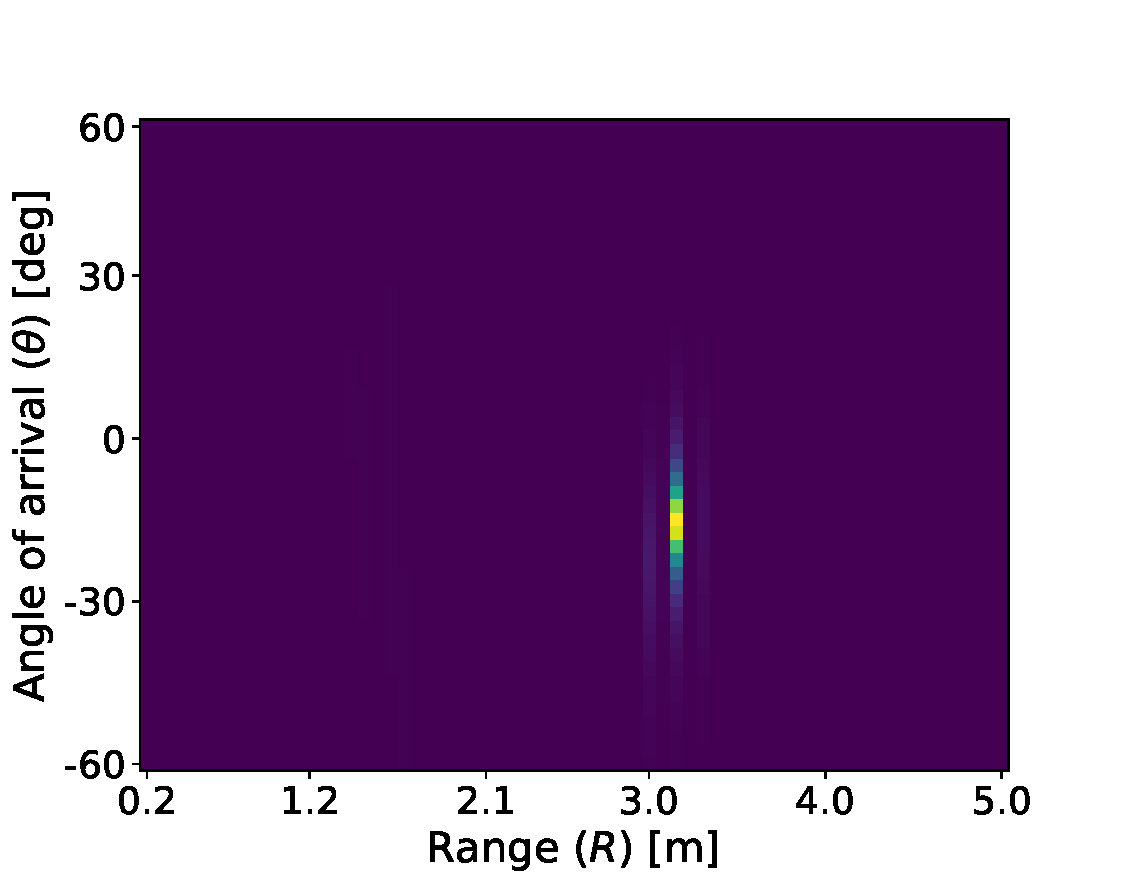
\includegraphics[width=\textwidth]{fig/4/music_spectrum.pdf}
        \caption{2-D MUSIC spectrum}
    \end{subfigure}
    \hfill
    \begin{subfigure}[b]{0.49\textwidth}
        \centering
        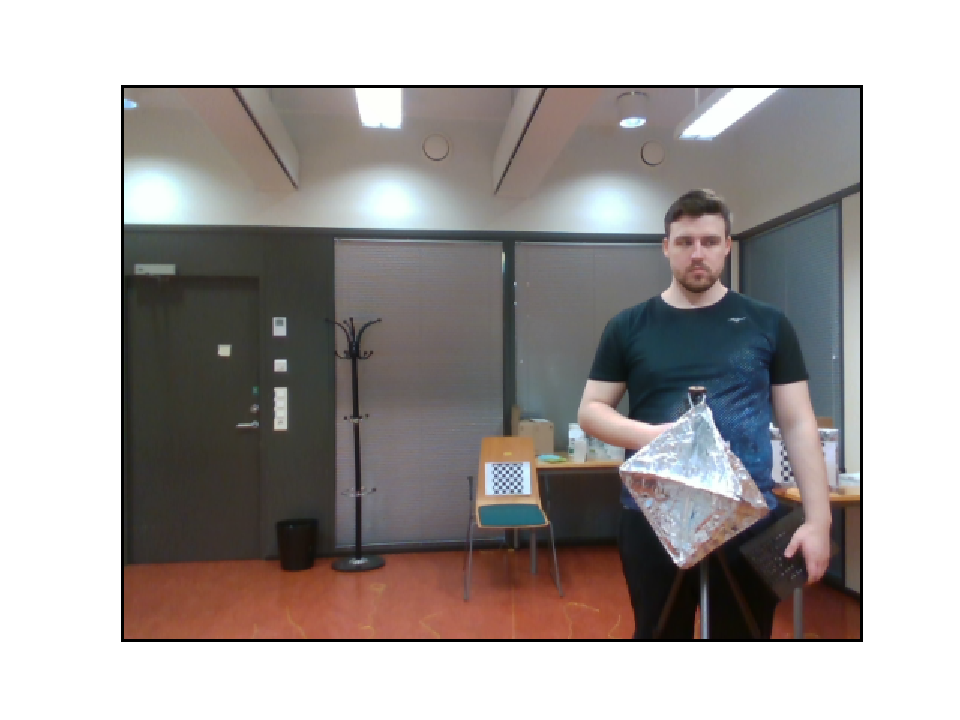
\includegraphics[width=\textwidth]{fig/4/music_corresponding_rgb_image.pdf}
        \caption{Corresponding RGB video frame}
    \end{subfigure}
    \caption{2D-MUSIC spectrum and a corresponding RGB video frame}
    \label{fig:2d-music-example}
\end{figure}

\subsection{Range-velocity spectrum}
\label{sec:doppler-spectrum}
The change in the range of a target, or a change in the propagation distance of the reflecting signal,
causes a phase shift in the received reflection.
This change is proportional to the change in the propagation distance.
Because the time between two samples is known,
the change in phase between two samples is therefore proportional to the velocity of the target.
When the velocity of the target $v \ll \frac{cM}{f T_{c}}$,
the relation between the phase shift and velocity is given by equation \ref{eq:phase-velocity-relation}
(derived in Appendix \ref{app:deriving-range-velocity-fft}).

\begin{equation}
    \label{eq:phase-velocity-relation}
    \Delta \phi = \frac{4 \pi f v T_{c}}{c}
\end{equation}

The equation \ref{eq:phase-velocity-relation} could be used to create a velocity steering vector
and the \gls{2d-music} algorithm could applied to acquire the range-velocity spectrum.
The \gls{music} algorithm is computationally very demanding, though,
and by taking multiple samples of the signal, a sufficient resolution can be had
for the range and velocity spectra even with the computationally much faster \gls{2d-fft} method.

Given the signal is sampled $N$ times per each of the $M$ chirps on $K$ channels,
the dimensions of the resulting data cube are $K \times M \times N$ (Section \ref{sec:radar-data}).
For the \gls{2d-fft} method,
the range and velocity resolutions ($\Delta R$ and $\Delta v$ respectively),
the maximum range ($R_{\mathrm{max}}$),
and the minimum and maximum velocities 
($v_{\mathrm{min}}$ and $v_{\mathrm{max}}$ respectively) are given by equations
\ref{eq:2dfft-range-resolution}--\ref{eq:2dfft-min-max-velocity}
(derived in Appendix \ref{app:deriving-range-velocity-fft}).

\begin{equation}
    \label{eq:2dfft-range-resolution}
    \Delta R = \frac{F_{s} c}{2NS}
\end{equation}
\begin{equation}
    \label{eq:2dfft-velocity-resolution}
    \Delta v = \frac{c}{2 M f T_{c}}
\end{equation}
\begin{equation}
    \label{eq:2dfft-max-range}
    R_{\mathrm{max}} = \frac{f_{s} c}{2 S}
\end{equation}
\begin{equation}
    \label{eq:2dfft-min-max-velocity}
    \begin{cases}
    v_{\mathrm{min}} = \frac{c}{4 f T_{c}} \\
    v_{\mathrm{max}} = - \frac{c}{4 f T_{c}}
    \end{cases}
\end{equation}

The range-velocity spectrum is calculated by first averaging the data
cube corresponding to the $y$:th frame ($\vec{S}_{y}$)
along the first axis (receivers) to increase the \gls{snr},
which will result in the data matrix $\vec{D}$, as given by equation \ref{eq:fft-snr-boost}.
The dimensions of $\vec{D}$ are $M \times N$.

\begin{equation}
    \label{eq:fft-snr-boost}
    \vec{D}(m, n) = \sum \limits_{k = 0}^{K-1} \vec{S}(k, m, n)
\end{equation}

After calculating $\vec{D}$, the Fourier transform is performed on the second axis of the matrix,
which is the fast-time samples. Denoting $\vec{D} = \begin{bmatrix} \vec{f}(0) & \vec{f}(1) & \ldots & \vec{f}(M-1) \end{bmatrix}$,
where $\vec{f}(m)$ is the vector containing the fast-time samples for the $m$:th chirp,
the operation is given by equation \ref{eq:fast-time-fft}.

\begin{equation}
    \label{eq:fast-time-fft}
    \vec{v}(m) = \mathcal{F} \left\{ \vec{f}(m) \right\}
\end{equation}

The operation $\mathcal{F} \{ \cdot \}$ in equation \ref{eq:fast-time-fft} is the discrete Fourier transform.
The resulting vector $\vec{\hat p}$ has contains the Fourier transform of $f(m)$ as its $m$:th element.
Each bin in the vectors $\vec{\hat p}$ corresponds to a range as given by equation \ref{eq:fast-time-fft-range}.
The function $R(n)$ gives the corresponding range for the $n$:th bin in vector $\vec{\hat p}(m)$ (Appendix \ref{app:deriving-range-velocity-fft}).

\begin{equation}
    \label{eq:fast-time-fft-range}
    R(n) = n \Delta R = \frac{n F_{s} c}{2NS}
\end{equation}

Assuming the range of the target changes by less than half a wavelength between two chirps,
the phase difference between the $n$:th element (frequency component) of vectors $\vec{\hat p}(m)$ and $\vec{\hat p}(m+1)$
is dictated by the distance the target has moved (Appendix \ref{app:deriving-range-velocity-fft}).
Thus, denoting $\vec{\hat P} = \begin{bmatrix} \vec{\hat p}(0) & \vec{\hat p}(1) \ldots & \vec{\hat p}(m-1) \end{bmatrix}^T$,
the Fourier transform can be applied along the first dimension of $\vec{\hat P}$ to acquire the velocities of the targets.
The range-velocity power-spectrum can thus be denoted as 
$\vec{P}^{\prime}$ as given by equation \ref{eq:slow-time-fft-matrix},
where $\vec{p}^{\prime}(n)$ is given by equation \ref{eq:slow-time-fft}.

\begin{equation}
    \label{eq:slow-time-fft-matrix}
    \vec{P}^{\prime} = \begin{bmatrix} \vec{p}^{\prime}(0) & \vec{p}^{\prime}(1) & \ldots & \vec{p}^{\prime}(n-1)\end{bmatrix}
\end{equation}

\begin{equation}
    \label{eq:slow-time-fft}
    \vec{p}^{\prime}(n) = \mathcal{F} \left \{ \begin{bmatrix} \vec{\hat P}(0, n) & \vec{\hat P}(1, n) & \ldots \vec{\hat P}(m-1, n) \end{bmatrix}^T \right \}
\end{equation}

Because the velocity can be either positive or negative, the matrix $\vec{P}^{\prime}$ still needs to be shifted so
that the zero-velocity bin is in the center.
The shifted range-velocity spectrum can be defined as $\vec{P}$ as given by equation \ref{eq:fft-shift}.

\begin{equation}
    \label{eq:fft-shift}
    \begin{cases}
        \forall m < \frac{M}{2} : \vec{P}(m, n) = \vec{P}^{\prime}(m + \frac{M}{2}, n) \\
        \forall m \ge \frac{M}{2} : \vec{P}(m, n) = \vec{P}^{\prime}(m - \frac{M}{2}, n) \\
    \end{cases}
\end{equation}

The velocity corresponding to the $m$:th bin on the first axis of $\vec{P}$ ($v(m)$) can be calculated from the 
minimum velocity and velocity resolution (equations \ref{eq:2dfft-min-max-velocity} and \ref{eq:2dfft-max-range}).
The velocity $v(m)$ is given by equation \ref{eq:slow-time-fft-bin-velocity}.

\begin{equation}
    \label{eq:slow-time-fft-bin-velocity}
    v(m) = -\frac{c}{4 f T_{c}} + \frac{m c}{2 M f T_{c}}
\end{equation}

Therefore, the matrix $\vec{P}$ contains the range-velocity spectrum of the radar cube.
The power of the reflection in element $\vec{P}(n, m)$ is the absolute value of the element,
whereas the range and velocity are given by equations 
\ref{eq:fast-time-fft-range} and \ref{eq:slow-time-fft-bin-velocity} respectively.
Figure \ref{fig:range-velocity-unfiltered} shows an example range-velocity spectrum
and Figure \ref{fig:range-velocity-rgb} shows the corresponding RGB image.
The target is walking away from the sensor, thus the velocity is negative.

\begin{figure}[H]
    \centering
    \begin{subfigure}[b]{0.49\textwidth}
        \centering
        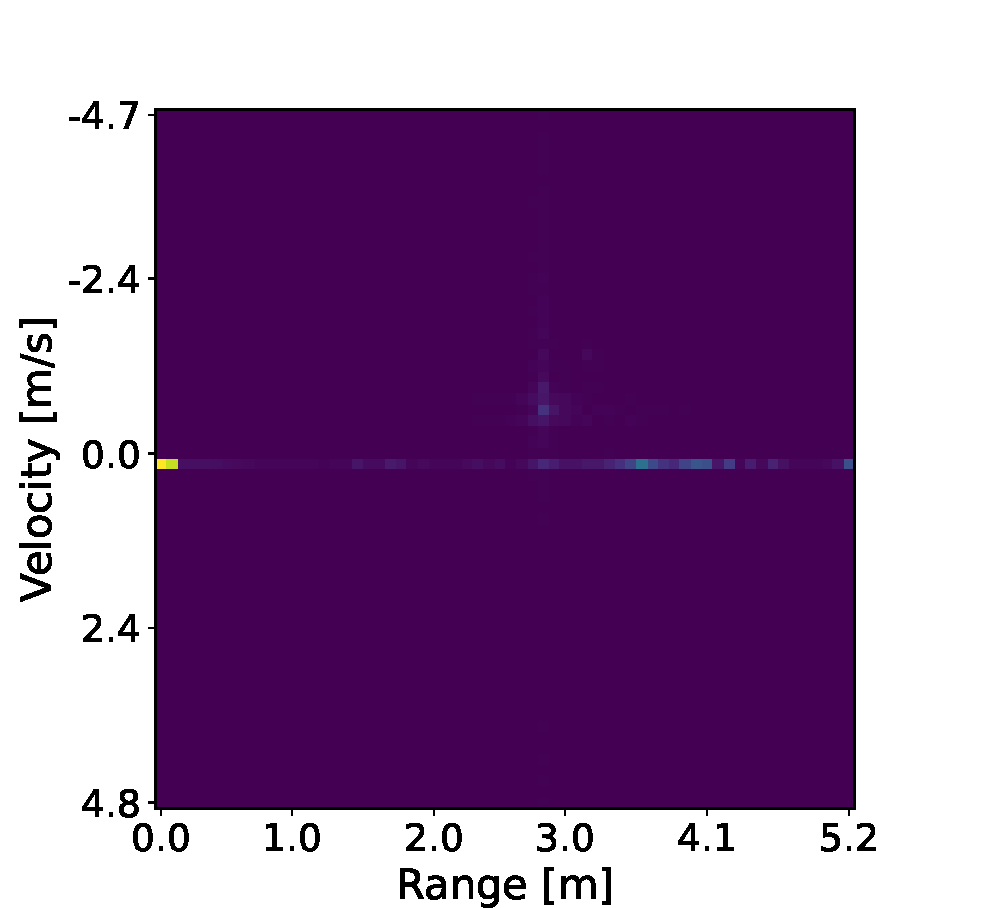
\includegraphics[width=\textwidth]{fig/4/range-velocity.pdf}
        \caption{Range-velocity spectrum}
        \label{fig:range-velocity-unfiltered}
    \end{subfigure}
    \hfill
    \begin{subfigure}[b]{0.49\textwidth}
        \centering
        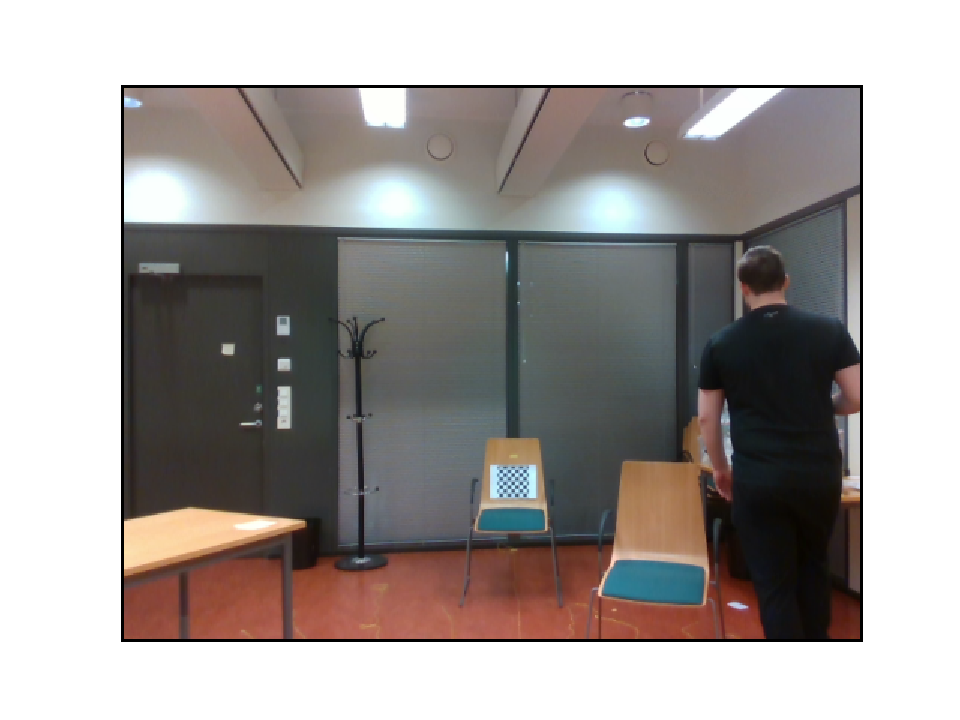
\includegraphics[width=\textwidth]{fig/4/range-velocity-rgb.pdf}
        \caption{Corresponding RGB video frame}
        \label{fig:range-velocity-rgb}
    \end{subfigure}
    \caption{
        Range-velocity spectrum and the corresponding RGB video frame.
    }
\end{figure}

It is seen from Figure \ref{fig:range-velocity-unfiltered} that there is a lot of power on the near-zero range and in the zero-velocity bins.
The near-zero range power is caused by self-interference and oscillator phase-noise in the radar.
Static clutter appears in the zero-velocity bins.
The first few range bins should always be attenuated and if only moving targets are of interest,
also the zero-velocity bins should be attenuated.

Attenuating can be done by defining vectors $\vec{u}$ and $\vec{v}$ of magnitudes $N$ and $M$ respectively,
where $\vec{u}(n)$ is the amplification of the $n$:th range bin
and $\vec{v}(m)$ is the amplification of the $m$:th velocity bin.
Corresponding diagonal matrices $\vec{U}$ and $\vec{V}$ can then be defined with the elements
of $\vec{u}$ and $\vec{v}$ along their diagonals.
Given a minimum range of interest $R_{\mathrm{min}}$,
the vectors $\vec{u}$ and $\vec{v}$ can be defined via equations
\ref{eq:range-coefficients} and \ref{eq:velocity-coefficients}.
The only velocity bins that are muted are the ones corresponding to zero-velocity.

\begin{equation}
\label{eq:range-coefficients}
    \begin{cases}
        \forall n \leq \left \lfloor \frac{ R_{\mathrm{min}} }{ \Delta R } \right \rfloor :
            \vec{u}(n) = 0 \\
        \forall n > \left \lfloor \frac{ R_{\mathrm{min}} }{ \Delta R } \right \rfloor :
            \vec{u}(n) = 1
    \end{cases}
\end{equation}

\begin{equation}
\label{eq:velocity-coefficients}
    \begin{cases}
        \forall m = \frac{1}{2}M :
            \vec{v}(m) = 0 \\
        \forall m \neq \frac{1}{2}M :
            \vec{v}(m) = 1
    \end{cases}
\end{equation}

Having defined the matrices $\vec{U}$ and $\vec{V}$ according to equations
\ref{eq:range-coefficients} and \ref{eq:velocity-coefficients},
the attenuation of the unwanted bins is achieved by multiplying the matrix
$\vec{P}$ with matrices $\vec{U}$ and $\vec{V}$ as given by equation \ref{eq:2dfft-attenuation}.
The Figure \ref{fig:range-velocity-spectrum-filtered} shows the velocity spectrum 
from Figure \ref{fig:range-velocity-unfiltered}, but with only the zero-range noise filtered 
in Figure \ref{fig:range-velocity-range-filtered} and both zero-range noise and zero-velocity clutter
filtered in Figure \ref{fig:range-velocity-both-filtered}.

\begin{equation}
    \label{eq:2dfft-attenuation}
    \vec{P}_{\mathrm{filtered}} = \vec{V} ( \vec{U} \vec{P}^T )^T
\end{equation}

\begin{figure}[H]
    \centering
    \begin{subfigure}[b]{0.49\textwidth}
        \centering
        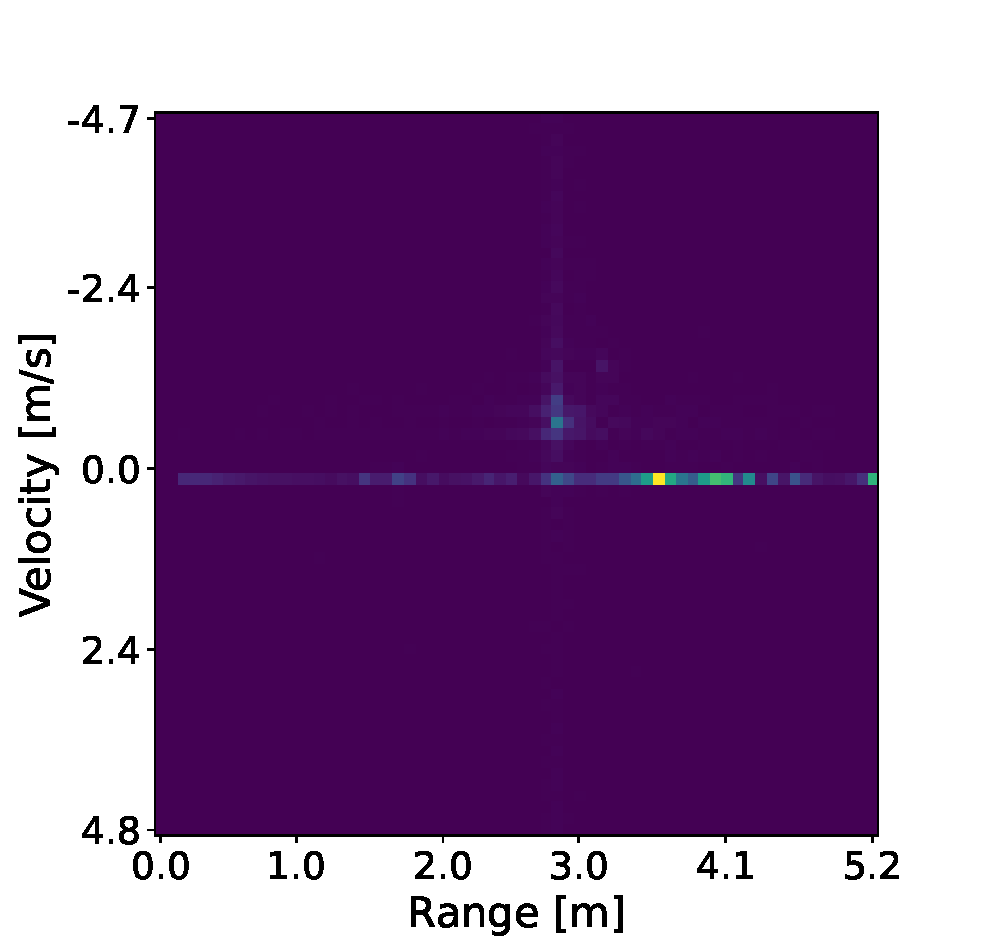
\includegraphics[width=\textwidth]{fig/4/range-velocity-range-filtered.pdf}
        \caption{Range-velocity spectrum with only zero-range noise filtered}
        \label{fig:range-velocity-range-filtered}
    \end{subfigure}
    \hfill
    \begin{subfigure}[b]{0.49\textwidth}
        \centering
        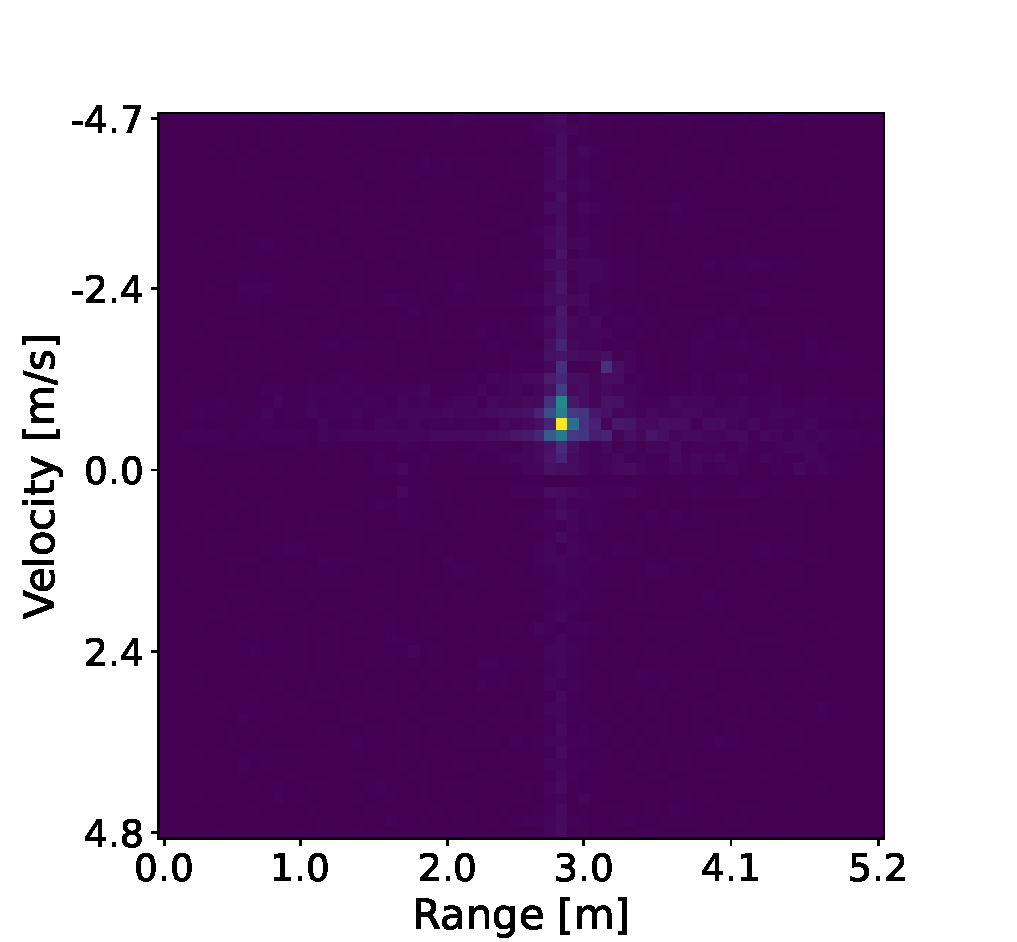
\includegraphics[width=\textwidth]{fig/4/range-velocity-both-filtered.pdf}
        \caption{Range-velocity spectrum with zero-range noise and zero-velocity clutter filtered}
        \label{fig:range-velocity-both-filtered}
    \end{subfigure}
    \caption{Filtered range-velocity spectrum}
    \label{fig:range-velocity-spectrum-filtered}
\end{figure}

An example implementation of the \gls{2d-fft} algorithm for acquiring and filtering the range-velocity spectrum
is presented in Appendix \ref{app:2dfft-range-velocity-example}. The example is written in Python.

\subsection{Target detection and tracking}
\label{sec:cfar}
From the calculated spectra, targets can be detected using target detection algorithms.
The most common way of detecting targets from the spectra is picking a threshold and checking if the power a cell is over it.
The threshold be picked in such a way that is higher than the noise power to minimize false positives.
The threshold must also be lower than the power reflected from targets in order to detect true positives. 
In other words, the threshold must be picked in such a way that the error rate is minimized, as illustrated by Figure \ref{fig:error-matrix}.

\begin{figure}
    \centering
    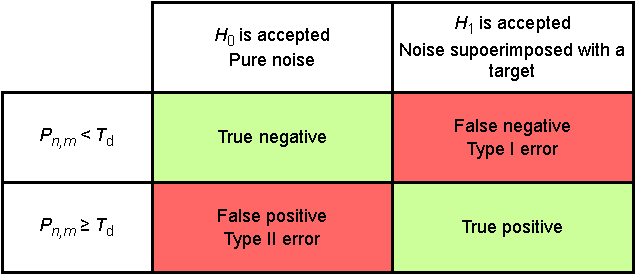
\includegraphics{fig/4/error-matrix.pdf}
    \caption{Different kinds of detection errors. The signal power in the test cell is denoted as $Y$, whereas $T$ is the detection threshold.}
    \label{fig:error-matrix}
\end{figure}

Formally, the target detection is done via hypothesis testing, where $H_0$ is that the cell contains only noise
and $H_1$ is that the cell contains noise superimposed with a target.
When the power of the tested cell is denoted as $Y$ and detection threshold as $T$,
the hypothesis test is defined by equation \ref{eq:hypothesis-test}.

\begin{equation}
    \label{eq:hypothesis-test}
    \begin{cases}
        H_{0}: Y < T \\
        H_{1}: Y \ge T
    \end{cases}
\end{equation}

The threshold depends on parameters of the noise-only distribution.
If the noise distribution was completely known prior to testing,
picking a correct detection threshold would be a trivial task.
In real-world applications the noise spectrum is space-time variant and therefore cannot be known a priori.
This leaves two choices for picking the detection threshold:
using distribution-free detection procedures \cite{distribution-free-detection} 
or estimating the noise spectrum and using an adaptive algorithm \cite{mean-level-detection}.

Typically a category of adaptive algorithms called \gls{cfar} detection algorithms is applied for detecting the targets.
The principle of \gls{cfar} algorithms is that the noise distribution is estimated from the calculated spectra (e.g. range-velocity or range-azimuth),
whereof the probability distribution for noise power is estimated.
The detection threshold is picked from the estimated noise probability distribution
based on a predefined probability of a false alarm, thus giving a false alarm rate that is constant.

When the probability density function for noise power is denoted as $f_{Y_0}(y)$,
the probability that $H_0$ is rejected when the power of the test cell $y$
is in the pure noise space $Y_0$
is given by the Neyman-Pearson criterion (equation \ref{eq:neyman-pearson}) \cite{fast-two-dimensional-cfar, neyman-pearson}.
The criterion is illustrated by Figure \ref{fig:neyman-pearson}.

\begin{equation}
    \label{eq:neyman-pearson}
    P_{\mathrm{fa}} = P(Y_0 \ge T) = \int_{T}^{\infty} f_{Y_0}(y)dy
\end{equation}

\begin{figure}
    \centering
    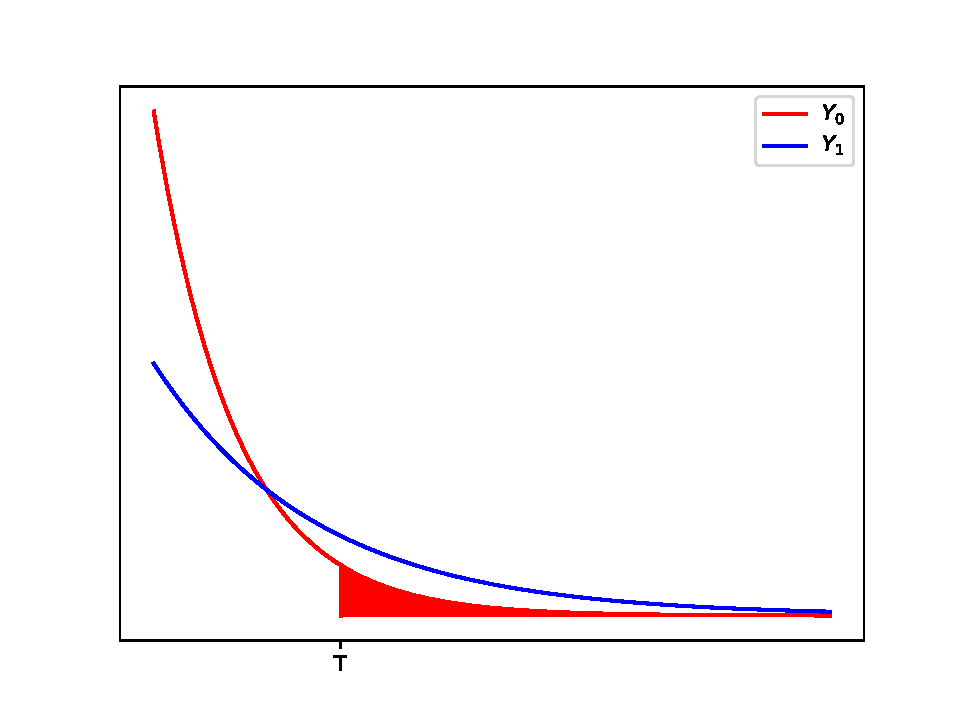
\includegraphics[width=0.67\textwidth]{fig/4/neyman-pearson.pdf}
    \caption{
        The probability density functions for the noise space $Y_0$ and signal space $Y_1$.
        The highlighted area is the probability of a false alarm as given by equation \ref{eq:neyman-pearson}
        for given decision threshold $T$.
    }
    \label{fig:neyman-pearson}
\end{figure}

When a square law detector is used for detecting targets in the signal,
i.e. the power of the signal is used as decision criterion,
and the noise in each cell is narrowband Gaussian noise,
the probability distribution for noise follows the exponential distribution.
Thus, the decision threshold $T$ is given by the quantile function of the exponential distribution (equation \ref{eq:exponential-quantile-func}),
where $\mu$ is the average noise power. \cite{mean-level-detection}

\begin{equation}
    \label{eq:exponential-quantile-func}
    T = -\mu \cdot \ln( 1-P_{\mathrm{fa}} )
\end{equation}

Different \gls{cfar} algorithms differ from each other in how the mean noise power $\mu$ is estimated.
The \gls{ca} \gls{cfar} algorithm assumes that the noise power in in each cell independent and identically distributed.
Based on the central limit theorem, the average noise power may be estimated by defining a window with sufficiently large dimensions,
and calculating the average power in the cells inside the window, disregarding the test cell and some guard cells around it.
This method is based on the assumption that the average noise power is calculated from cells that have a very high likelihood of containing purely noise.
The assumption is fair when the targets are sparse.

The estimated average noise power $\hat \mu$ around the cell $(y_0, y_1)$
in the \gls{ca} \gls{cfar} algorithm is given by the equation \ref{eq:ca-cfar-noise-estimate}.
The term $Z(y_0, y_1)$ and $G(y_0, y_1)$ in the equation are the sum power of the $A \times B$
observation window around the test cell (equation \ref{eq:observation-window-sum})
and the sum power of the $C \times D$ guard cells around the test cell
(equation \ref{eq:guard-window-sum}) respectively.
The terms $N$ and $M$ are the dimensions of the $N \times M$ matrix that is the power spectrum $\vec{P}$,
given by the equations \ref{eq:2d-music-spectrum} and \ref{eq:fft-shift}. \cite{fast-two-dimensional-cfar}
The test cell and the surrounding windows are illustrated by Figure \ref{fig:ca-cfar-window}.

\begin{align}
    \label{eq:ca-cfar-noise-estimate}
    & \hat \mu (y_0, y_1) = \frac{1}{AB-CD} \left( Z(y_0, y_1) - G(y_0, y_1) \right)
    \\
    \label{eq:observation-window-sum}
    & Z(y_0, y_1) = \sum_{a=a_{\mathrm{min}}}^{a_{\mathrm{max}}}\sum_{b=m_{\mathrm{min}}}^{b_{\mathrm{max}}} \vec{P}(a, b) 
    \\
    & a_{\mathrm{min}} = \max \left( y_{0}- \lfloor A/2 \rfloor , 0 \right) \quad a_{\mathrm{max}} = \min \left( N, y_{0}+ \lfloor A/2 \rfloor \right)
    \\
    & b_{\mathrm{min}} = \max \left( y_{1}- \lfloor B/2 \rfloor , 0 \right) \quad b_{\mathrm{max}} = \min \left( M, y_{0}+ \lfloor B/2 \rfloor  \right)
    \\
    \label{eq:guard-window-sum}
    & G(y_0, y_1) = \sum_{c=c_{\mathrm{min}}}^{c_{\mathrm{max}}}\sum_{d=d_{\mathrm{min}}}^{d_{\mathrm{max}}} \vec{P}(c, d) 
    \\
    & c_{\mathrm{min}} = \max \left( y_{0}- \lfloor C/2 \rfloor , 0 \right) \quad c_{\mathrm{max}} = \min \left( N, y_{0}+ \lfloor C/2 \rfloor  \right)
    \\
    & d_{\mathrm{min}} = \max \left( y_{1}- \lfloor D/2 \rfloor , 0 \right) \quad d_{\mathrm{max}} = \min \left( M, y_{0}+ \lfloor D/2 \rfloor  \right)
\end{align}

It is noteworthy that the \gls{2d-music} algorithm (equation \ref{eq:2d-music-spectrum} does not produce a true power spectrum,
but rather a pseudo-power spectrum where the cells contain a correlation number instead of actual signal power.
Thus, the noise pseudo-power may not in reality be exponentially distributed and another distribution or a target detection algorithm
is likely better suited for the task.

\begin{figure}
    \centering
    \begin{subfigure}[b]{0.3\textwidth}
        \centering
        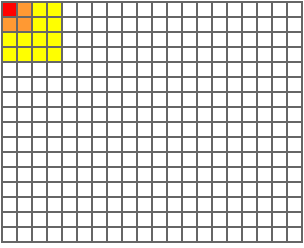
\includegraphics[width=\textwidth]{fig/4/ca-cfar-window-1.pdf}
        \caption{$(y_0, y_1) = (0, 0)$}
    \end{subfigure}
    \hfill
    \begin{subfigure}[b]{0.3\textwidth}
        \centering
        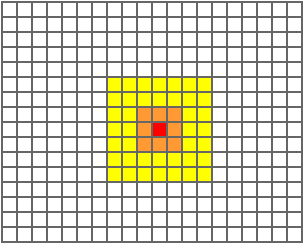
\includegraphics[width=\textwidth]{fig/4/ca-cfar-window-2.pdf}
        \caption{$(y_0, y_1) = (N/2, M/2)$}
    \end{subfigure}
    \hfill
    \begin{subfigure}[b]{0.3\textwidth}
        \centering
        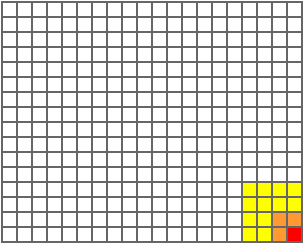
\includegraphics[width=\textwidth]{fig/4/ca-cfar-window-3.pdf}
        \caption{$(y_0, y_1) = (N-1, M-1)$}
    \end{subfigure}
    \caption{
        The observation window, guard cells and test cell in the Cell Averaging Constant False Alarm Rate algorithm.
        The test cell is highlighted in red, guard cells in orange, and noise estimation window in yellow.
        In all cases, the noise estimation window has dimensions $7 \times 7$ and the guard window has dimensions $3 \times 3$.
    }
    \label{fig:ca-cfar-window}
\end{figure}

In a multitarget situation, the average noise power estimate of \gls{ca} \gls{cfar} is no longer a good estimate,
as it is skewed from targets appearing inside the noise estimating window.
The average noise level is thus estimated too high and weak targets are "masked" by nearby strong targets,
which causes type \rom{2} errors ($H_0$ is erroneously accepted).
The \gls{os} \gls{cfar} algorithm may be deployed in multi-target situations to achieve better detection performance. \cite{nato-radar-topics}

In the \gls{os} \gls{cfar} algorithm, the powers of the cells inside the observation window are sorted in smallest-first order.
The $l$:th element is then picked from the sorted array and used as the average noise power estimate.
Given the observation window has dimensions $A \times B$, based on the work of Rohling, a reasonable value for is $l = \frac{3}{4}AB$.
In the \gls{os} \gls{cfar} algorithm, the guard cells are omitted.
\cite{radar-cfar-thresholding-in-clitter-and-multiple-target-situations}
The figure \ref{fig:cfar-plots} illustrates the results of applying the \gls{ca} and \gls{os} \gls{cfar} algorithms
on the range-velocity and range-angle spectra. The range-angle spectrum is calculated via the \gls{2d-music} algorithm whereas the range-velocity
spectrum is calculated via \gls{2d-fft}.
It is apparent from figure \ref{fig:os-cfar-music} that the exponentially distributed noise power assumption may not be good for the \gls{2d-music} spectrum.
The effects of masking in the \gls{ca} \gls{cfar} algorithm can be seen by comparing figures \ref{fig:ca-cfar-fft} and \ref{fig:os-cfar-fft}.

\begin{figure}[H]
    \centering
    \begin{subfigure}{0.49\textwidth}
        \centering
        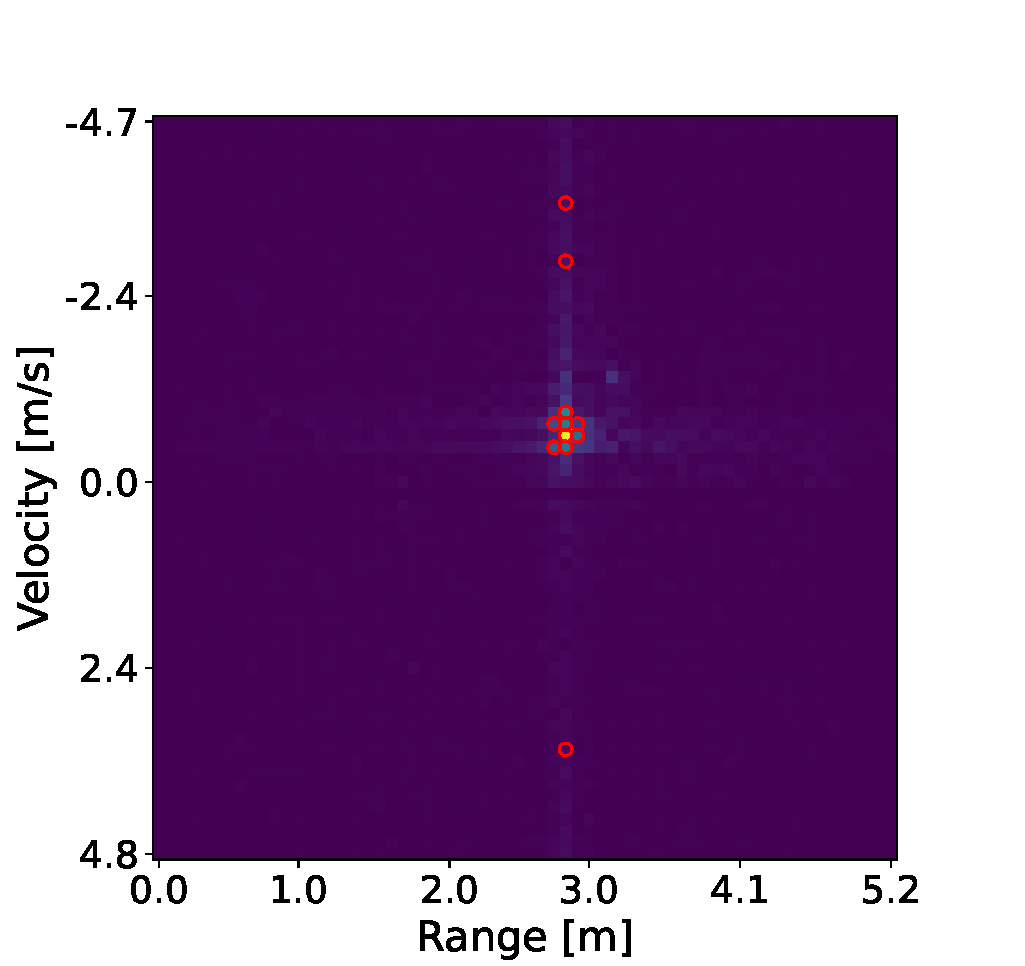
\includegraphics[width=\textwidth]{fig/4/ca-cfar-fft.pdf}
        \caption{CA CFAR applied on range-velocity spectrum calculated via FFT.}
        \label{fig:ca-cfar-fft}
    \end{subfigure}
    \hfill
    \begin{subfigure}{0.49\textwidth}
        \centering
        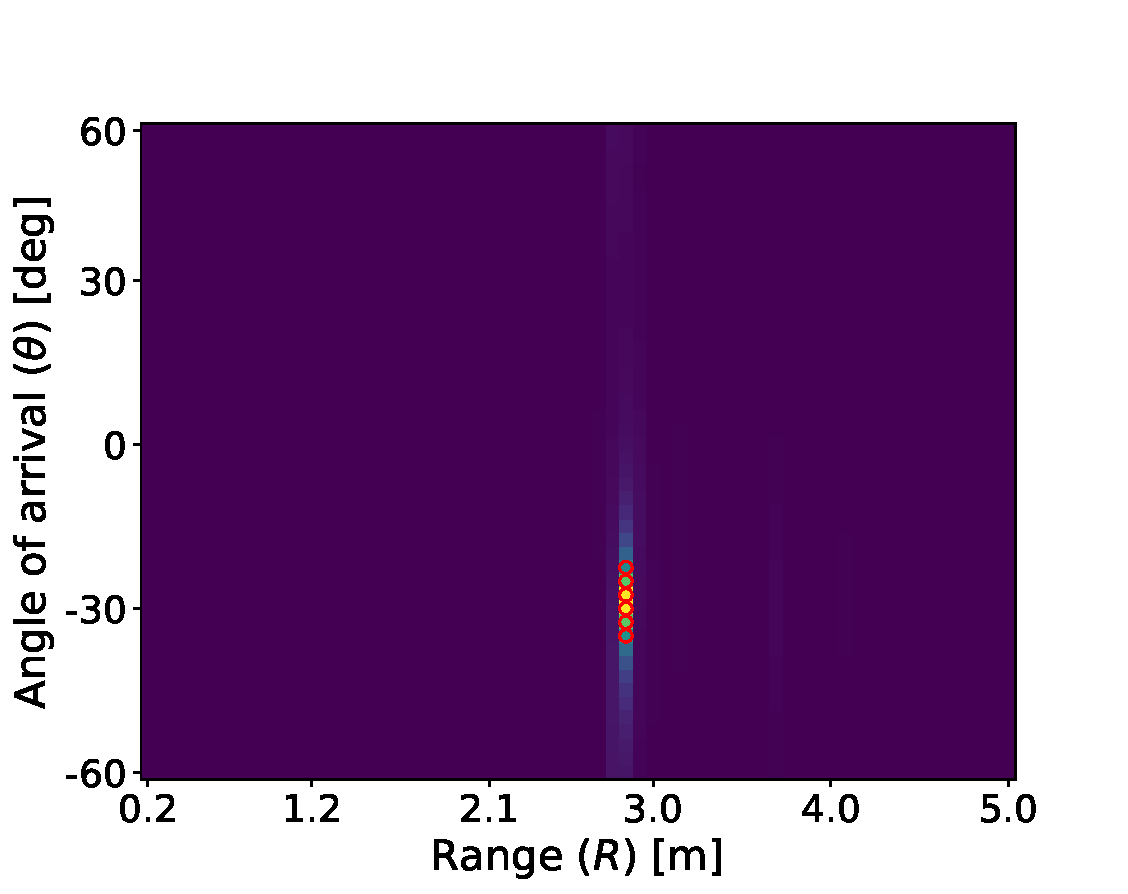
\includegraphics[width=\textwidth]{fig/4/ca-cfar-music.pdf}
        \caption{CA CFAR applied on range-angle spectrum calculated via 2D-MUSIC.}
        \label{fig:ca-cfar-music}
    \end{subfigure}
    \vskip\baselineskip
    \begin{subfigure}{0.49\textwidth}
        \centering
        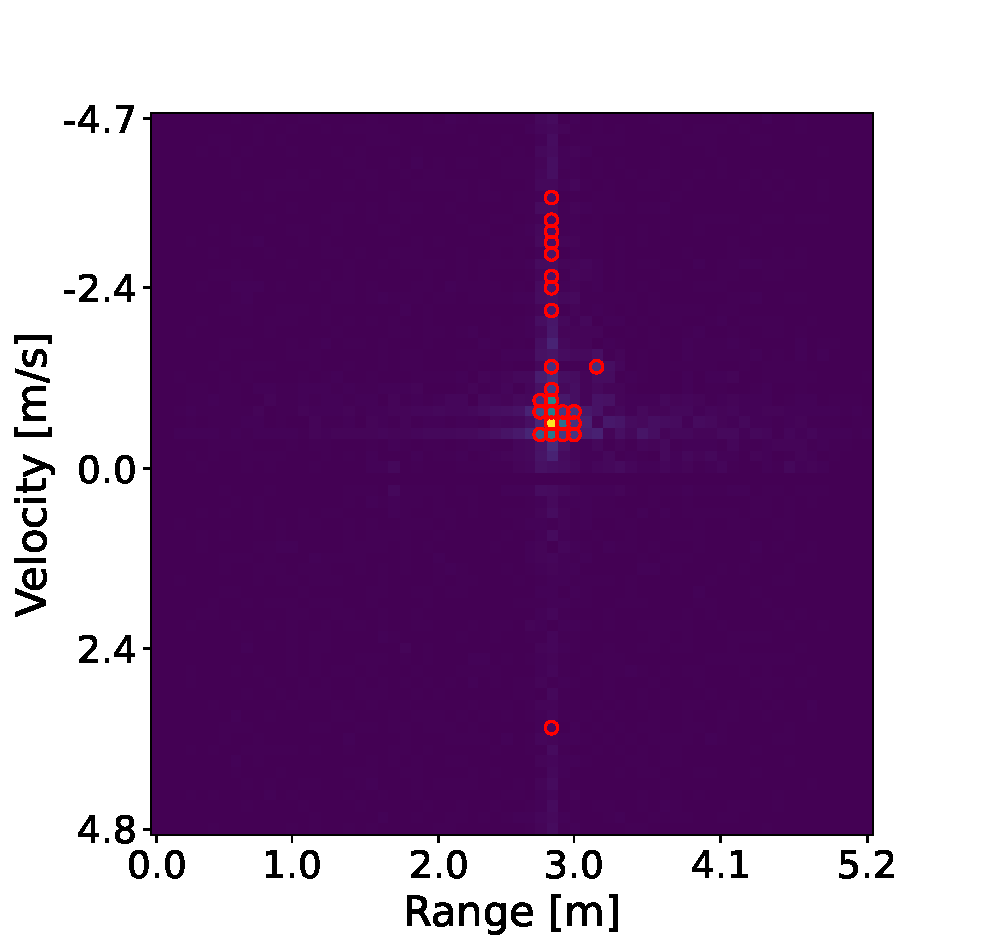
\includegraphics[width=\textwidth]{fig/4/os-cfar-fft.pdf}
        \caption{OS CFAR applied on range-velocity spectrum calculated via FFT.}
        \label{fig:os-cfar-fft}
    \end{subfigure}
    \hfill
    \begin{subfigure}{0.49\textwidth}
        \centering
        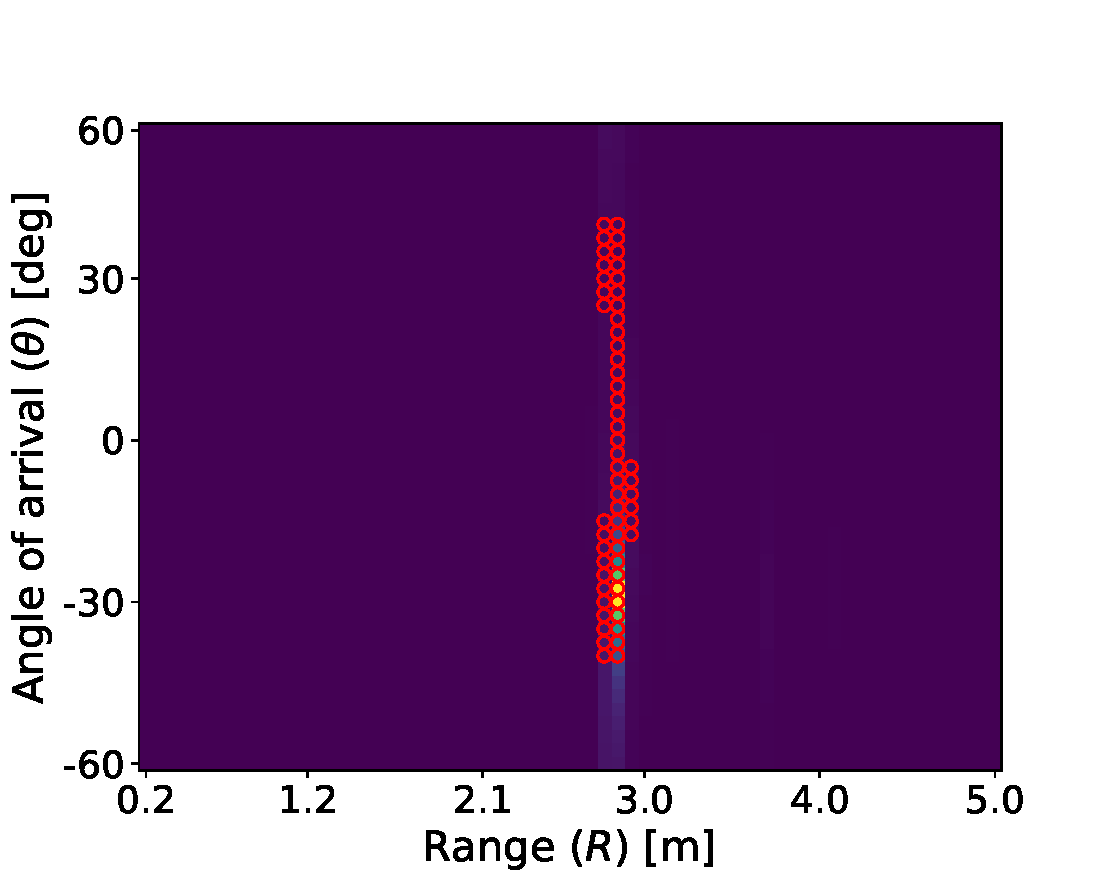
\includegraphics[width=\textwidth]{fig/4/os-cfar-music.pdf}
        \caption{OS CFAR applied on range-angle spectrum calculated via 2D-MUSIC:}
        \label{fig:os-cfar-music}
    \end{subfigure}
    \caption{
        The Cell Averaging and Ordered Statistic Constant False Alarm Rate algorithms applied on the range-velocity and range-angle spectra.
        The figures are scaled show the amplitude of the spectrum rather than power.
    }
    \label{fig:cfar-plots}
\end{figure}

In addition to the basic \gls{ca} and \gls{os} \gls{cfar} algorithms, multiple variations and combinations of the two have been developed over the years.
The \gls{ca} and \gls{os} \gls{cfar} still serve as the basis for most of the variations.
The variations typically consider different computational complexity, noise distribution,
target amplitude statistics, and multiple target situations. \cite{nato-radar-topics}

After target detection, target tracking algorithms may be used to track the same target between multiple frames.
With target tracking, the track of a single target may be recorded and predicted
and the appearance of new targets and the disappearance of old targets may be detected.
Additionally, when the velocity spectrum of a single target can be recorded through multiple frames,
this information can be used for \gls{har}.

Target tracking can be split into two parts: track filtering and measurement-to-track association.
The first part considers predicting the possible target tracks to determine the possible locations for a target in upcoming frames.
The latter part considers assigning measurements (detected targets) to predicted paths.
For track filtering, Kalman filtering is a popular choice.
For measurement-to-track association, nearest-neighbour filtering or probabilistic models are commonly used. \cite{modern-radar-1}

\section{Depth camera record}   
\label{sec:depth-file}
The depth camera record is stored in the \texttt{depth.raw} file.
The recording program produces two bytes of output per pixel.
The output represents the measured distance at the pixel in millimeters as a 16-bit integer number (short int).
The frame resolution and frame rate are stored in the \texttt{metadata.yaml} file.
Table \ref{tab:depth-metadata} documents the metadata fields recorded under the \texttt{camera.depth} section in \texttt{metadata.yaml} file.
\begin{table}
    \begin{tabular}{l l}
        \toprule
        \textbf{Key} & \textbf{Meaning} \\
        \midrule
        framerate & Number of recorded frames per second, decimal number \\
        resolution & Resolution of the stored frames, string representation of a list: \texttt{'[M, N]'} \\
        \bottomrule
    \end{tabular}
    \caption{Metadata fields for the depth camera}
    \label{tab:depth-metadata}
\end{table}

Given the resolution is $N \times M$ (height $\times$ width) and the recorded data is represented by $\vec{d}$,
where each element is two bytes long, the index of the $i$:th pixel of the $z$:th frame $\vec{f}_{j}(i)$ can be calculated using equation \ref{eq:depth-pixel}.

\begin{equation}
    \label{eq:depth-pixel}
    \forall i \in \left[ 0, NM-1 \right] \land z \in \left[ 0, \frac{| \vec{d} |}{NM}-1 \right] : \vec{f}_{z}(i) = \vec{d}(NMz+i)
\end{equation}

The frame $\vec{f}_z$ can then be rearranged as a matrix $\vec{F}_z$,
which represents the pixels of the image in such a way that the origin is in the upper left corner.
The pixel in coordinates $(n,m)$ in the frame $\vec{F}_z$ is given by the equation \ref{eq:pixel-in-frame-depth}.

\begin{equation}
    \label{eq:pixel-in-frame-depth}
    \forall n \in [0, N-1] \land m \in [0, M] : F_{z}(n,m) = \vec{f}_{z}(mN+n)
\end{equation}

Given the \gls{fov} of the sensor is $\Theta \times \Phi$ in the azimuth and altitude dimensions respectively,
the \gls{fov} of each subpixel is $\frac{\Theta}{N} \times \frac{\Phi}{M}$.
Given the angle is measured from the upper-left corner of a pixel and origin is in the center pixel,
the range (in given frame) $R_n$ measured at angle $(\theta, \phi)$ 
is given by equation \ref{eq:depth-range-angle}.
The term $1 \div 1000$ converts the measured range from millimeters to meters.

\begin{equation}
    \label{eq:depth-range-angle}
    \forall \theta \in \left[ -\frac{\Theta}{2}, \frac{\Theta}{2} \right] \land \phi \in \left[ -\frac{\Phi}{2}, \frac{\Phi}{2} \right] :
    R_z(\theta, \phi) =
    \frac{1}{1000} 
    \vec{F}_z \left(
        \left\lfloor \frac{N}{2} + \frac{N\theta}{\Theta} \right\rfloor ,
        \left\lfloor \frac{M}{2} + \frac{M\phi}{\Phi} \right\rfloor
    \right)
\end{equation}

\begin{figure}[H]
    \centering
    \begin{subfigure}[t]{0.49\textwidth}
        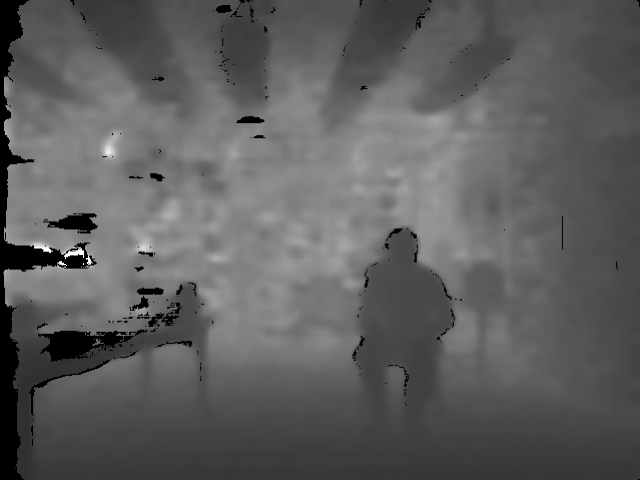
\includegraphics[width=\textwidth]{fig/4/depth-image.png}
        \caption{An example depth image.}
        \label{fig:depth-camera-frame}
    \end{subfigure}
    \hfill
    \begin{subfigure}[t]{0.49\textwidth}
        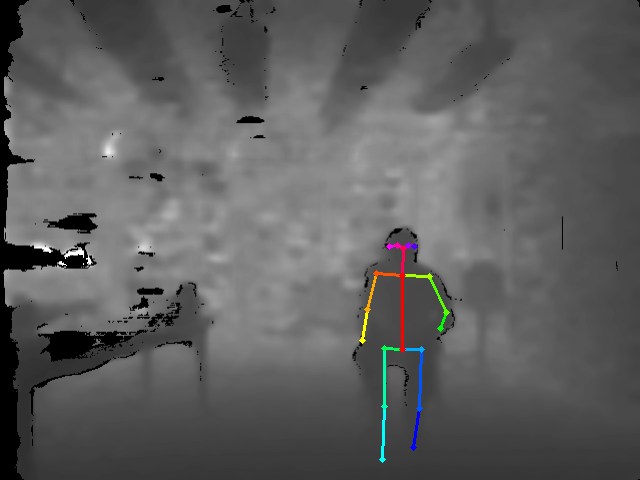
\includegraphics[width=\textwidth]{fig/4/depth-image-skeleton.png}
        \caption{Joint position information extracted from the depth image (PNG) using OpenPose\cite{openpose}.}
        \label{fig:depth-camera-frame-skeleton}
    \end{subfigure}
    \caption{Depth image extracted from the \texttt{depth.raw} file.}
\end{figure}

Appendix \ref{app:image-parsing} shows an example of parsing the depth camera frames from the recorded data.
An example of a resulting image is presented in Figure \ref{fig:depth-camera-frame}.
Machine learning models may be used to extract e.g. posture information from the depth images.
Example models include TexMesh\cite{tex-mesh}, A2J\cite{a2j}, and DoubleFusion\cite{double-fusion}.
Figure \ref{fig:depth-camera-frame-skeleton} shows an example of an image where the joint positions have been estimated using
OpenPose \cite{openpose} from the depth image that has been exported to PNG format and rendered to the image.

\section{RGB camera record}
\label{sec:rgb-file}
The RGB camera record is stored in the \texttt{rgb.raw} file.
The recording program produces three bytes of output per pixel. 
The bytes correspond to the red, green and blue values of the pixel,
such that the first byte tells the red value,
second byte tells the green value and the third byte tells the blue value.
Each byte represents an unsigned 8-bit integer.
The frame rate and resolution of the recording are stored in the \texttt{metadata.yaml} file
under the \texttt{camera.rgb} section.
Table \ref{tab:rgb-metadata} documents the metadata fields recorded for the RGB camera.

\begin{table}
    \begin{tabular}{l l}
        \toprule
        \textbf{Key} & \textbf{Meaning} \\
        \midrule
        framerate & Number of recorded frames per second, decimal number \\
        resolution & Resolution of the stored frames, string representation of a list: \texttt{'[M, N]'} \\
        \bottomrule
    \end{tabular}
    \caption{Metadata fields for the RBG camera}
    \label{tab:rgb-metadata}
\end{table}

Denoting the vector of bytes stored in the file as $\vec{b}$,
the data may be organized in pixels such that the $i$:th pixel $\vec{p}_{i}$ is given by equation \ref{eq:rgb-pixels}.
When the pixels have been parsed, given the resolution of the recording is $N \times M$ (height $\times$ width),
the $z$:th frame, denoted as $\vec{F}_z$ can be parsed based on equation \ref{eq:rgb-pixels-to-frames}.

\begin{align}
    \label{eq:rgb-pixels}
    \forall i \in \left[ 0, \frac{ | \vec{b} | }{3} \right] : \vec{p}_{i} = \begin{bmatrix} \vec{b}(3i) & \vec{b}(3i+1) & \vec{b}(3i+2) \end{bmatrix}^T
    \\
    \label{eq:rgb-pixels-to-frames}
    \forall z \in \left[ 0, \frac{|p|}{NM} \right] : \vec{F}_{z}(n, m) = \vec{p}(zNM + nM + m)
\end{align}

Appendix \ref{app:image-parsing} shows an example of parsing the RGB camera frames from the recorded data.
An example of a resulting image is presented in Figure \ref{fig:rgb-camera-frame}.
Machine learning models may be used to e.g. extract posture information or detect items from the RGB images.
Example models include ....
Figure \ref{fig:rgb-camera-frame-skeleton} shows an example of an image
where the joint positions have been estimated using OpenPose \cite{openpose}.

\begin{figure}[H]
    \centering
    \begin{subfigure}[t]{0.49\textwidth}
        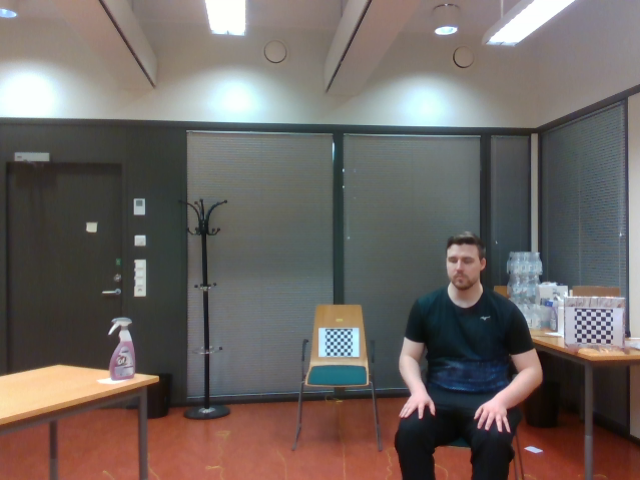
\includegraphics[width=\textwidth]{fig/4/rgb-image.png}
        \caption{An example RGB image.}
        \label{fig:rgb-camera-frame}
    \end{subfigure}
    \hfill
    \begin{subfigure}[t]{0.49\textwidth}
        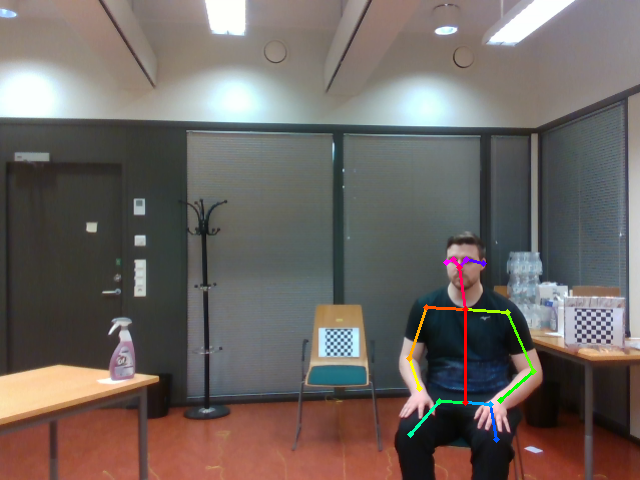
\includegraphics[width=\textwidth]{fig/4/rgb-image-skeleton.png}
        \caption{Joint position information extracted from the RGB using OpenPose\cite{openpose}.}
        \label{fig:rgb-camera-frame-skeleton}
    \end{subfigure}
    \caption{RGB image extracted from the \texttt{rgb.raw} file.}
\end{figure}

\section{Microphone samples}
\label{sec:audio-file}
The microphone record is stored in the \texttt{audio.wav} file. 
The file contains 16 audio channels and the sampling rate is stored in the \texttt{metadata.yaml} file.
The sampling rate is also stored as metadata in the WAV file.
Table \ref{tab:mic-metadata} documents the metadata recorded for the audio file in the \texttt{metadata.yaml} file in the \texttt{audio} section.

\begin{table}[H]
    \centering
    \begin{tabular}{l l}
        \toprule
        \textbf{Key} & \textbf{Meaning} \\
        \midrule
        samplerate & The sampling frequency for the microphone recording, integer number. \\
        \bottomrule
    \end{tabular}
    \caption{Metadata recorded for the \texttt{audio.wav} file.}
    \label{tab:mic-metadata}
\end{table}

Figure \ref{fig:mic-channels} shows the positions of the microphones in the used MiniDSP UMA-16 microphone.
The microphone numbers correspond to the audio channel numbers such that MIC1 is channel 0, MIC2 is channel 1, etc.
Each sample in the data is represented by a 32-bit floating-point number.
The samples are real-valued.
Appendix \ref{app:mic-parsing} shows an example of reading the audio file with Python using the Soundfile \cite{python-soundfile} library.

\begin{figure}
    \centering
    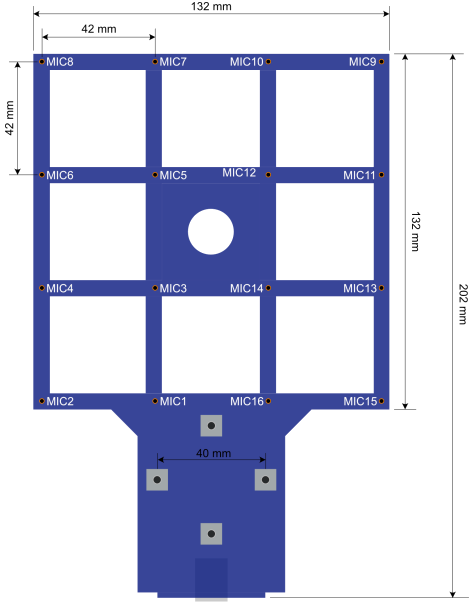
\includegraphics[width=0.67\textwidth]{fig/4/microphone-channels.png}
    \caption{Channels of the MiniDSP UMA-16 microphone \cite{minidsp-spec}.}
    \label{fig:mic-channels}
\end{figure}

